%! TEX root = ../main.tex
\documentclass[../main.tex]{subfiles}

\begin{document}

\section{Risultati}

Avendo preso le misure a partire da un'estremità della guida dentata la curva non ha il picco centrato in $y = 0$, quindi si è proceduto con il traslare le misure.
% L'errore attribuito a questa operazione è di $\qty{1}{\mm}$. %? review errore specifico per ogni fenditura?

A partire dai dati raccolti con apertura del sensore pari a $\qty{1.5}{\mm}$ 
è stata stimata la dimensione della fenditura utilizzando due metodi

\begin{enumerate}
    \item La posizione dei minimi ricavata graficamente che permette di ottenere la dimensione della fenditura utilizzando l'\autoref{eq:y=0 values}
    \item Il fit tramite l'\autoref{eq:fit}, in cui è stato inserito un parametro $c$ che permette di traslare la curva verticalmente in modo da tenere in considerazione la presenza di rumore.
\end{enumerate}

\begin{equation} \label{eq:fit}
    I(I_{0}, a, c) = I_{0} \; \sinc^{2} \left( \frac{\pi a}{\lambda} \cdot \frac{y}{L} \right) + c
\end{equation}

\subsection{Fenditura da $\mathbf{\qty{0.02}{\mm}}$}

Per la fenditura da $\qty{0.02}{\mm}$ ed apertura del sensore pari a $\qty{1.5}{\mm}$ sono stati raccolti $4$ set di dati che sono riportati in %\autoref{}.

\begin{figure}[ht!]
    \centering
    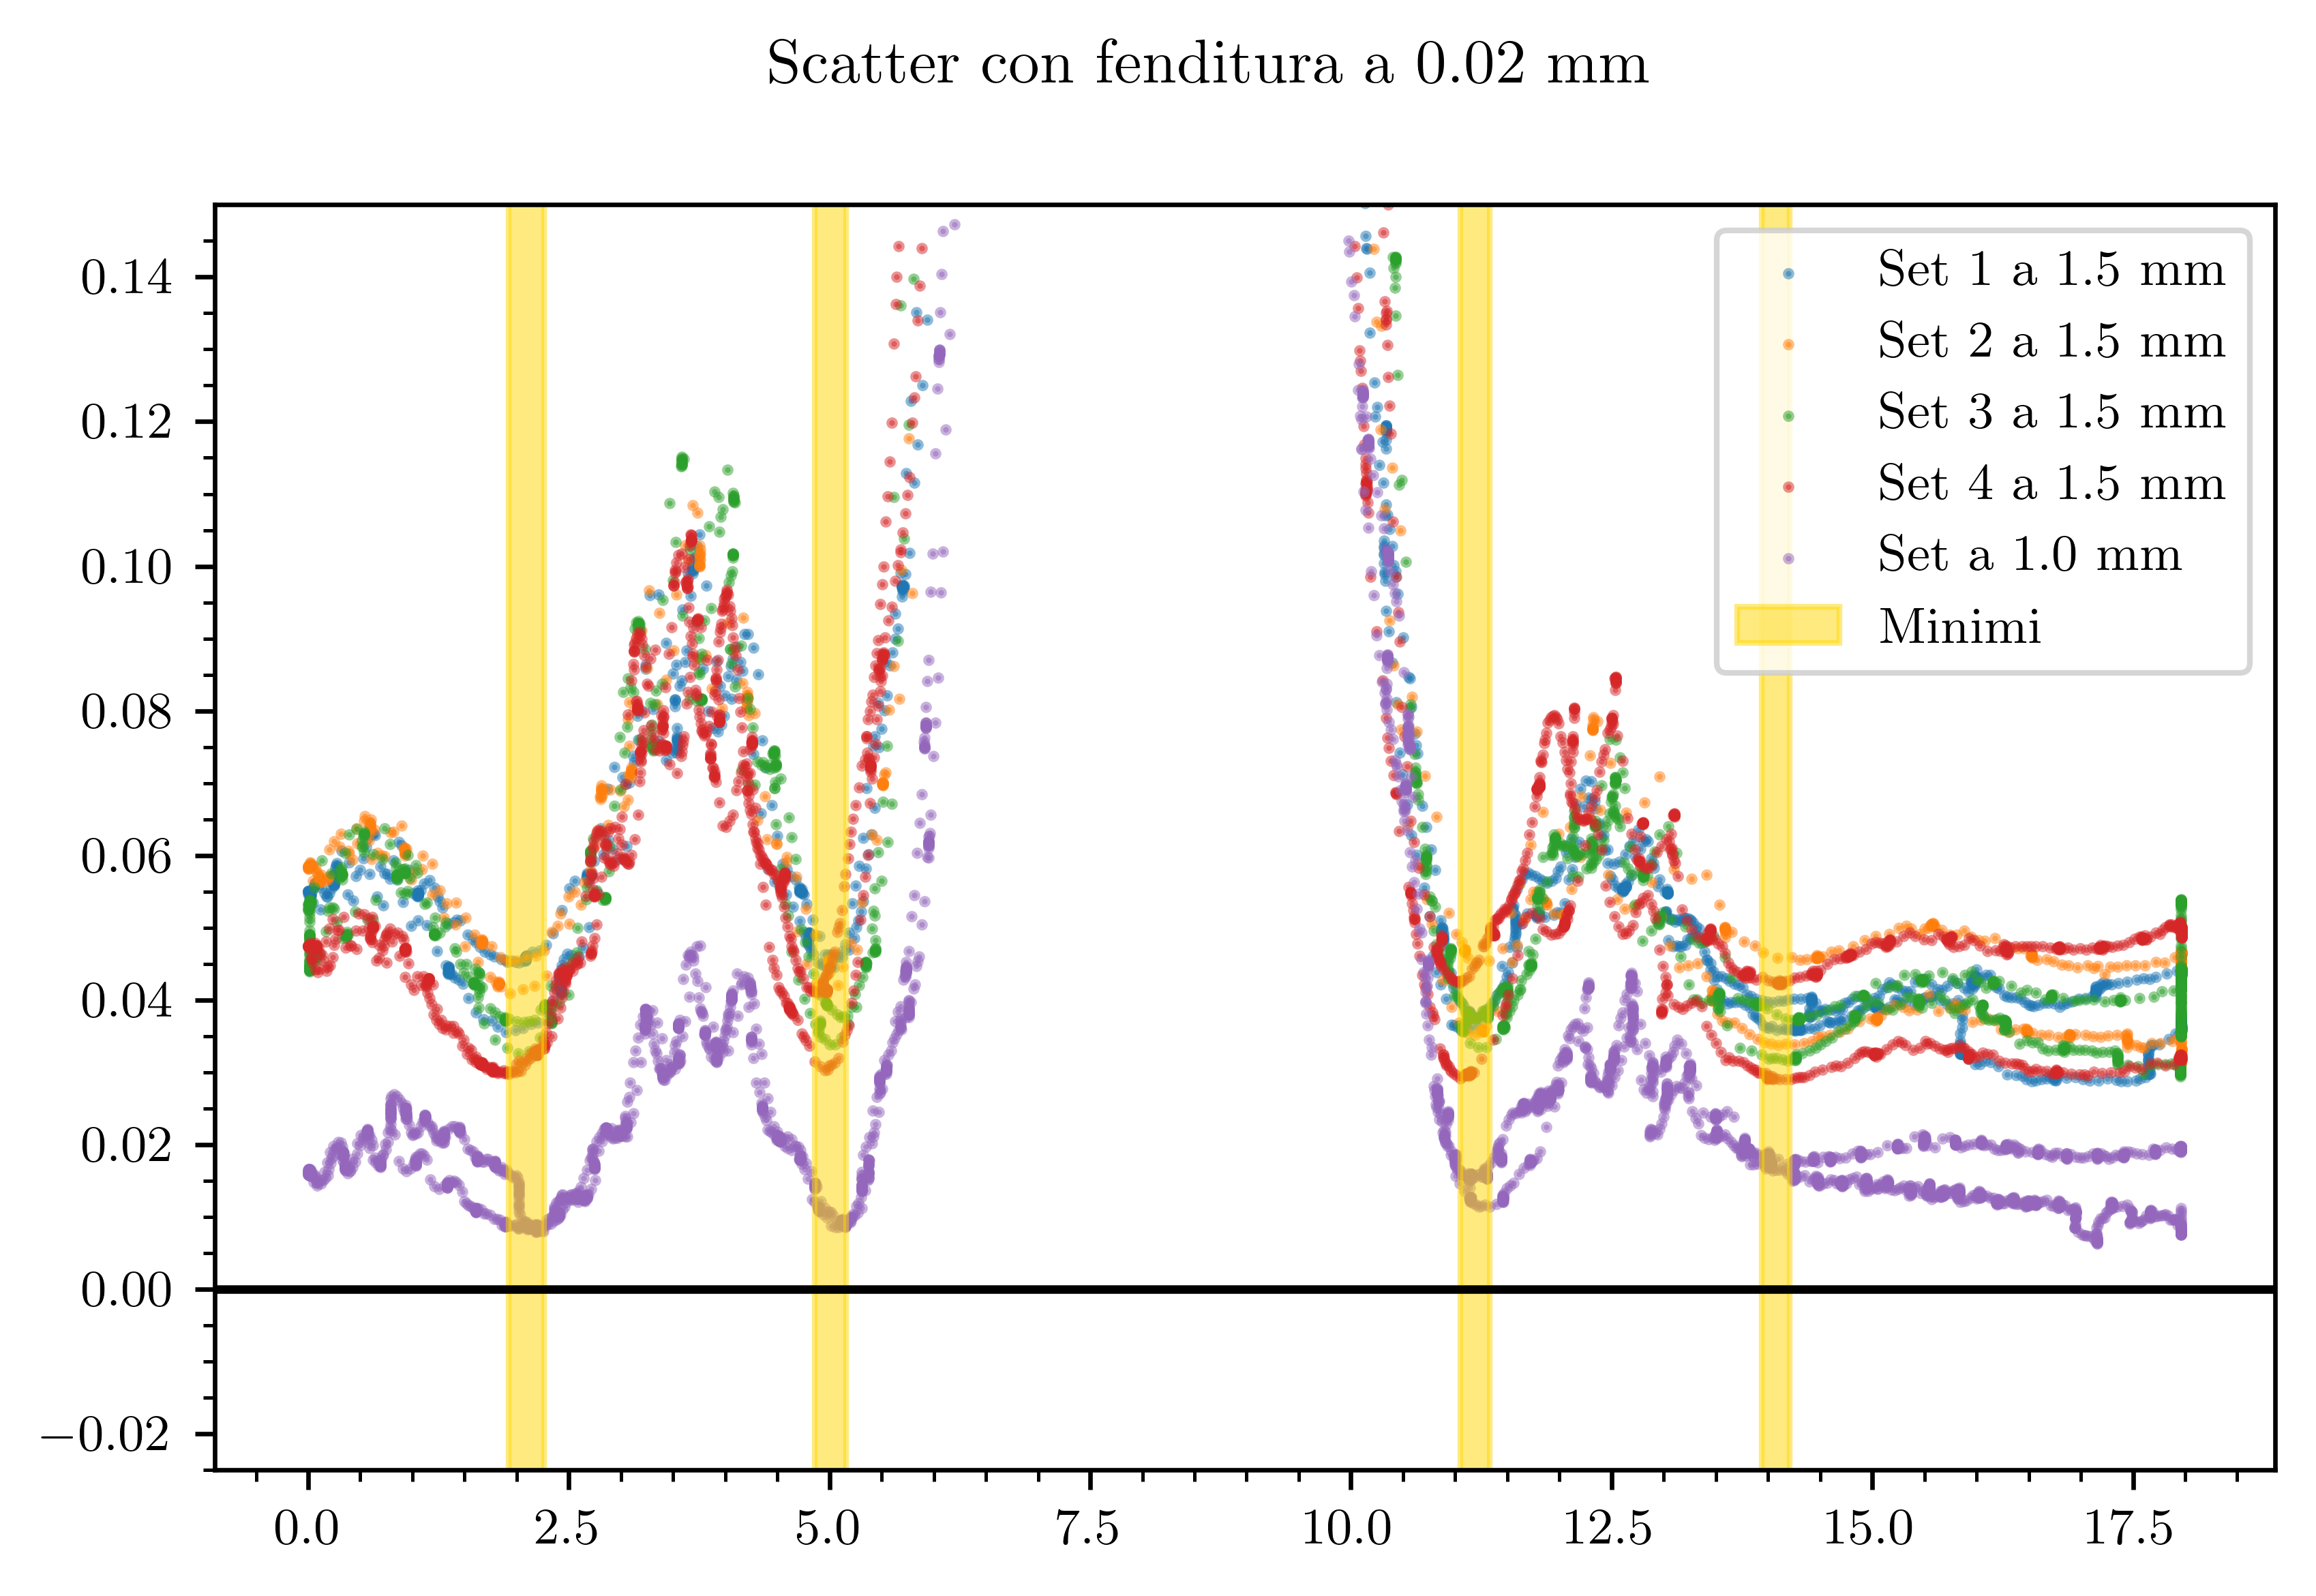
\includegraphics{min_0.02.png}
    \caption{Intensità luminosa $I$ in funzione della posizione $y$ del sensore (in metri) per la fenditura a $\qty{0.02}{\milli\metre}$. Si può notare un'asimmetria dei picchi  rispetto al centro. In figura sono segnati i minimi ricavati graficamente con i relativi errori. Su ciascun minimo si considera un errore di posizione di $\qty{1.0}{\mm}$, che contribuisce all'ampiezza di ciascuno degli intervalli evidenziati. È possibile notare un segnale a frequenza costante che si sovrappone alla figura di diffrazione.} % todo: aggiungere qualcosa in più alla descrizione+ commento asimmetria dati?
    \label{fig:minimi 0.02}
\end{figure}

Le posizioni dei minimi ottenute dalla \autoref{fig:minimi 0.02} sono riportate in \autoref{tab:minimi 0.02}.

\begin{table}[ht!]
    \centering
    \caption{Posizione dei minimi, ottenuta graficamente dalla \autoref{fig:minimi 0.02}, riportata di fianco al proprio indice $m$ ed al valore $\frac{\lambda L}{a} \; (\si{\metre})$ stimati seguendo l'\autoref{eq:y=0 values}. Il valore di $a$ derivato da ciascun minimo è stato ricavato con la formula inversa dopo aver posto $\lambda = \qty{650}{\nm}$ ed $L = \qty{98.5+-0.1}{\cm}$ sommando in quadratura i contributi all'errore di $\delta y$ e $\delta L$.}
    \begin{tabular}{r|cc|c}
        \toprule
        $m$  & $y \; (\si{\metre})$ & $\frac{\lambda L}{a} \; (\si{\metre})$ & $a \; (\si{\mm})$ \\
        \midrule
        $-2$ & \num{-0.061+-0.007} & \num{0.030+-0.003} & \num{0.021+-0.002} \\
        $-1$ & \num{-0.032+-0.004} & \num{0.032+-0.004} & \num{0.020+-0.003} \\
        $1$  & \num{0.031+-0.005}  & \num{0.031+-0.005} & \num{0.021+-0.003} \\
        $2$  & \num{0.061+-0.006}  & \num{0.030+-0.003} & \num{0.021+-0.002} \\
        \bottomrule
    \end{tabular}
    \label{tab:minimi 0.02}
\end{table}

Intersecando i valori di $a$ così ricavati si ottiene $a = \qty{0.021+-0.002}{\mm}$.

% Facendo una media pesata dei valori di $a$ ottenuti si ottiene $a = \qty{0.0209+-0.0012}{\mm}$. %? review: è meglio l'intersezione o la media?

\begin{figure}[ht!]
    \centering
    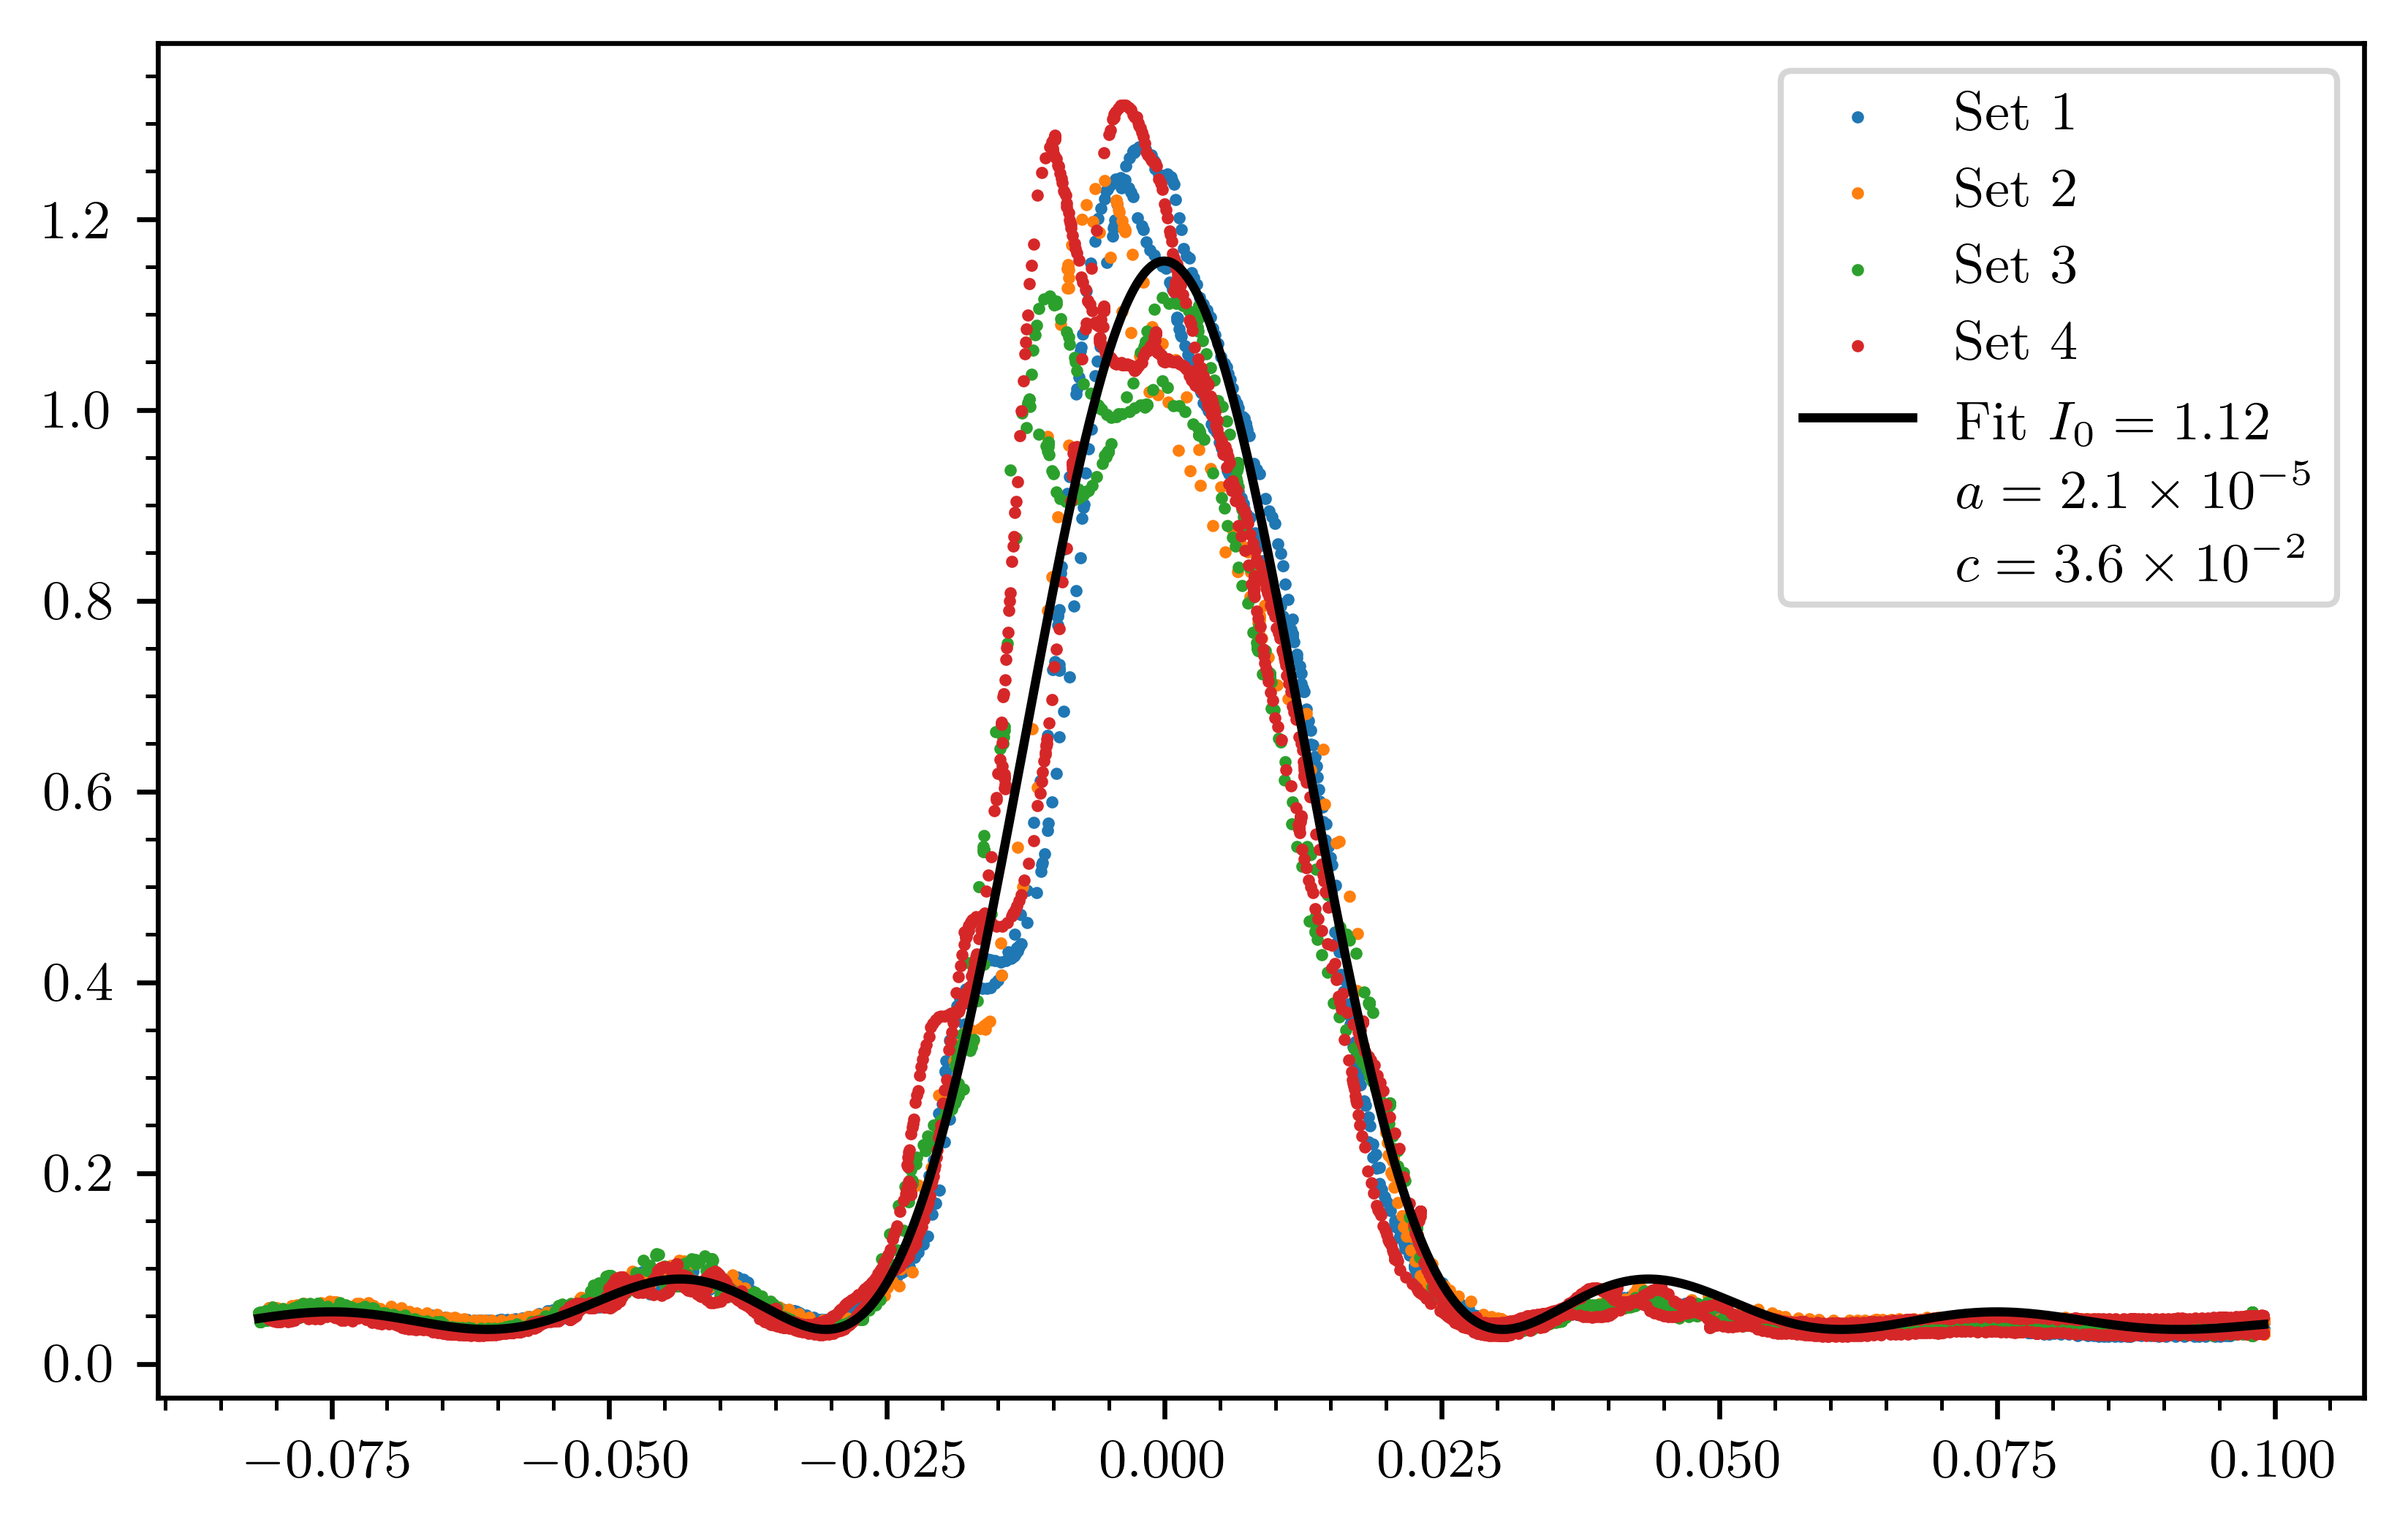
\includegraphics{fit_0.02.png}
    \caption{Intensità luminosa $I_{0}$ in funzione della posizione $y$ del sensore (in metri) per la fenditura a $\qty{0.02}{\mm}$. In figura è riportato il fit fatto utilizzando l'\autoref{eq:fit}. I valori dei parametri ottenuti sono $I_{0} = \num{1.12+-0.15}$, $a = \qty{0.021+-0.002}{\mm}$ e $c = \num{3.6+-0.8e-2}$.}
    \label{fig:fit 0.02}
\end{figure}

Sia il valore ottenuto col fit che il valore ottenuto dal grafico risultano compatibili con il valore teorico di $a$.

Per confrontare le misure ottenute con diverse aperture del sensore si è scelto di utilizzare il set $1$ delle misure con apertura $\qty{1.5}{\mm}$, in quanto è quello che meno presenta deformazioni lungo il picco centrale e ci permette di confrontare l'ampiezza di quest'ultimo.

\begin{figure}[ht!]
    \centering
    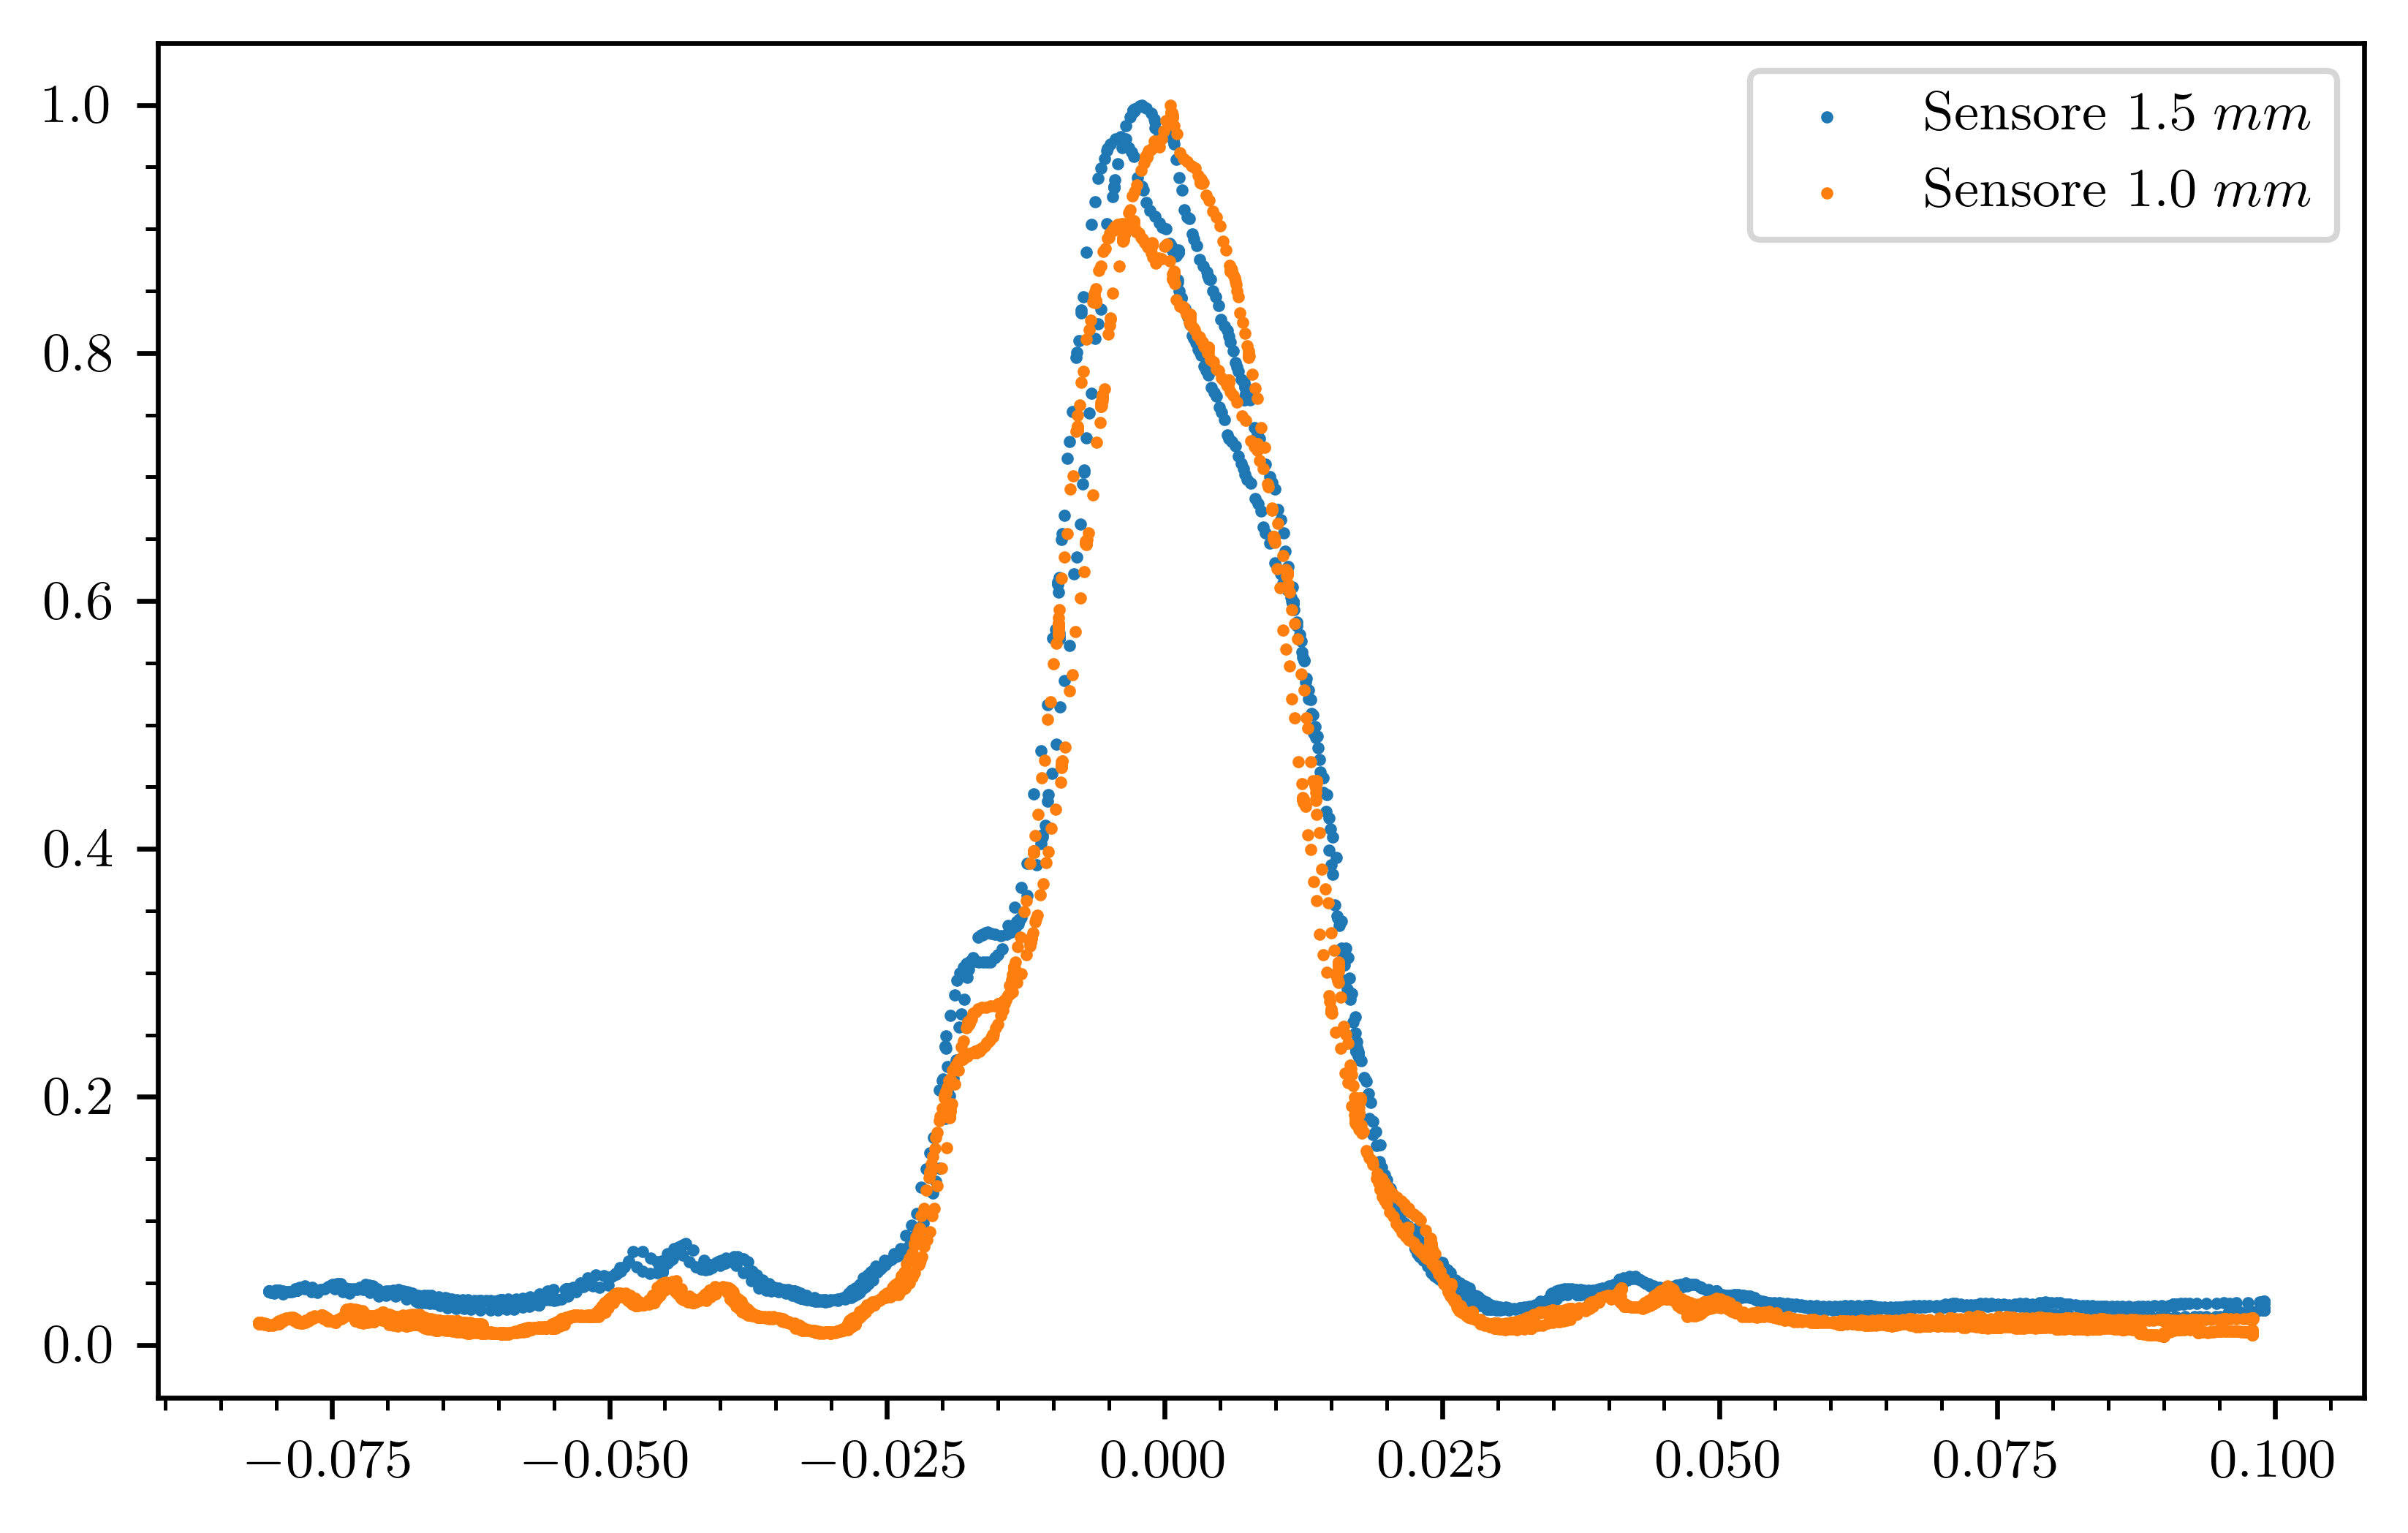
\includegraphics{sensor_0.02.png}
    \caption{Grafico dell'intensità luminosa relativa $I$ in funzione della posizione $y$ (in metri) per ciascuna delle due aperture del sensore.
    Riducendo l'apertura del sensore l'intensità misurata diminuisce permettendo di passare al fondo-scala più piccolo (\textit{candela}) per l'apertura da $\qty{1.0}{\mm}$.
    I valori delle intensità sono stati scalati in modo che l'altezza del picco centrale fosse pari a $1$, questo permette di confrontare i picchi con più semplicità. In effetti è possibile notare come la curva tracciata dalle misure con un'apertura più stretta abbia un picco centrale leggermente più schiacciato.
    Inoltre nelle code delle curve è evidente come il rumore di fondo diminuisca notevolmente, in particolar modo nel set di dati con il sensore a $\qty{1.0}{\mm}$. Questo potrebbe essere dovuto alla riduzione della luce che entra nel sensore o al cambio di fondo-scala, che porta ad una corrente di buio notevolmente inferiore.
    Come sarà possibile vedere in seguito la seconda ipotesi è quella che più si adatta ai dati raccolti.} %! quantificare di quanto si stringe il picco
    \label{fig:sensore 0.02}
\end{figure}

Si può notare che anche nei grafici \ref{fig:minimi 0.02} e \ref{fig:sensore 0.02} persiste il segnale di frequenza costante: questo potrebbe essere dato da un difetto della fenditura stessa, che causa un'interferenza la quale si sovrappone alla figura di diffrazione.

\newpage

\subsection{Fenditura $a = \qty{0.04}{\milli\metre}$}

\begin{figure}[ht!]
    \centering
    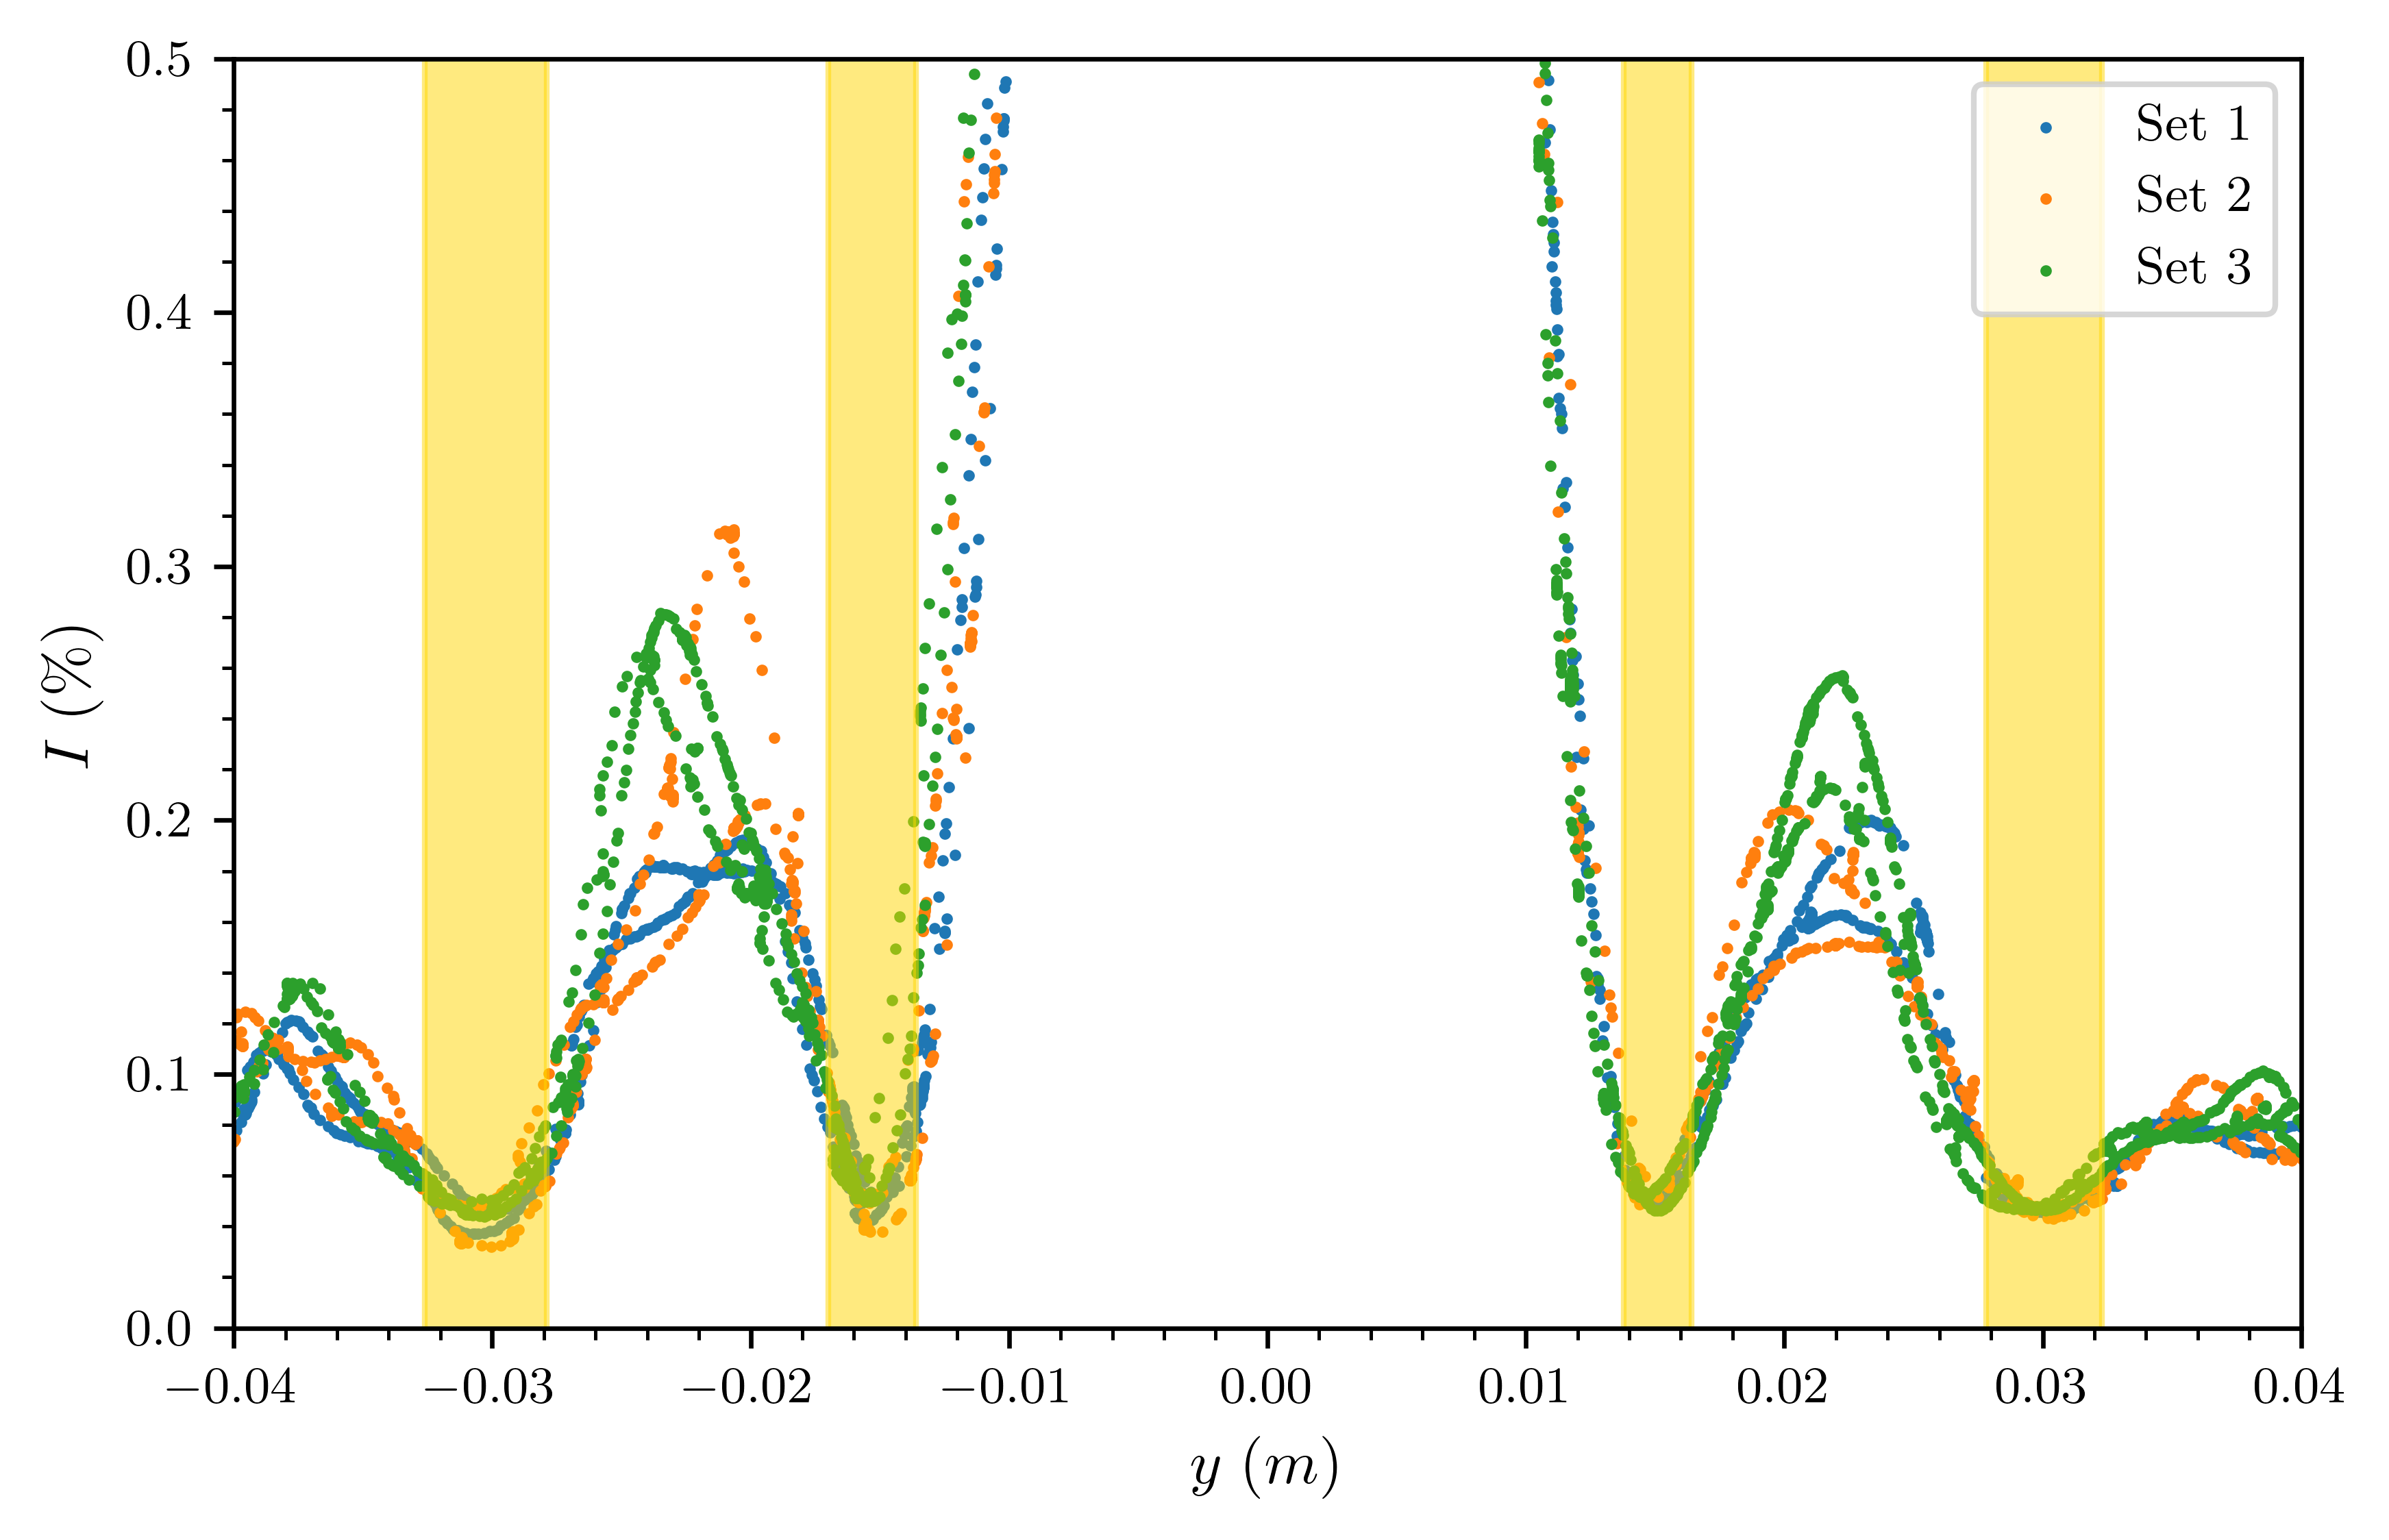
\includegraphics{min_0.04.png}
    \caption{Intensità luminosa $I$ in funzione della posizione $y$ del sensore (in metri) per la fenditura a $\qty{0.04}{\mm}$. I dati dei set 1 e 3 risultano quasi simmetrici, mentre il set 2 è visibilmente asimmetrico. In figura sono segnati i minimi ricavati graficamente con i relativi errori. Qui si considera un errore di posizione di $\qty{0.5}{\mm}$.} % todo: aggiungere qualcosa in più alla descrizione, trovare forse un motivo migliore per l'errore di 1mm
    \label{fig:minimi 0.04}
\end{figure}

Le posizioni dei minimi ottenute sono le seguenti:

\begin{table}[ht!]
    \centering
    \caption{}
    \begin{tabular}{r|cc|c}
        \toprule
        $m$  & $y \; (\si{\metre})$ & $\frac{\lambda L}{a} \; (\si{\metre})$ & $a \; (\si{\mm})$ \\
        \midrule
        $-2$ & $0.030 \pm 0.002$ & $0.0151 \pm 0.0011$ & \num{0.042+-0.003} \\
        $-1$ & $0.0153 \pm 0.0017$ & $0.0153 \pm 0.0017$ & \num{0.042+-0.005} \\
        $1$  & $0.0151 \pm 0.0013$ & $0.0151 \pm 0.0013$ & \num{0.042+-0.004} \\
        $2$  & $0.030 \pm 0.002$ & $0.0150 \pm 0.0011$ & \num{0.043+-0.003} \\
        \bottomrule
    \end{tabular}
    \label{tab:minimi 0.04}
\end{table}

Intersecando le barre d'errore dei valori ottenuti si ha $a = \qty{0.043+-0.003}{\mm}$.

% Prendendo in considerazione la somma delle barre d'errore dei valori ottenuti $a = \qty{0.043+-0.004}{\mm}$.

% Facendo una media pesata dei valori ottenuti si ha $a = \qty{0.0424+-0.0012}{\mm}$. %? media o intersezione

\begin{figure}[ht!]
    \centering
    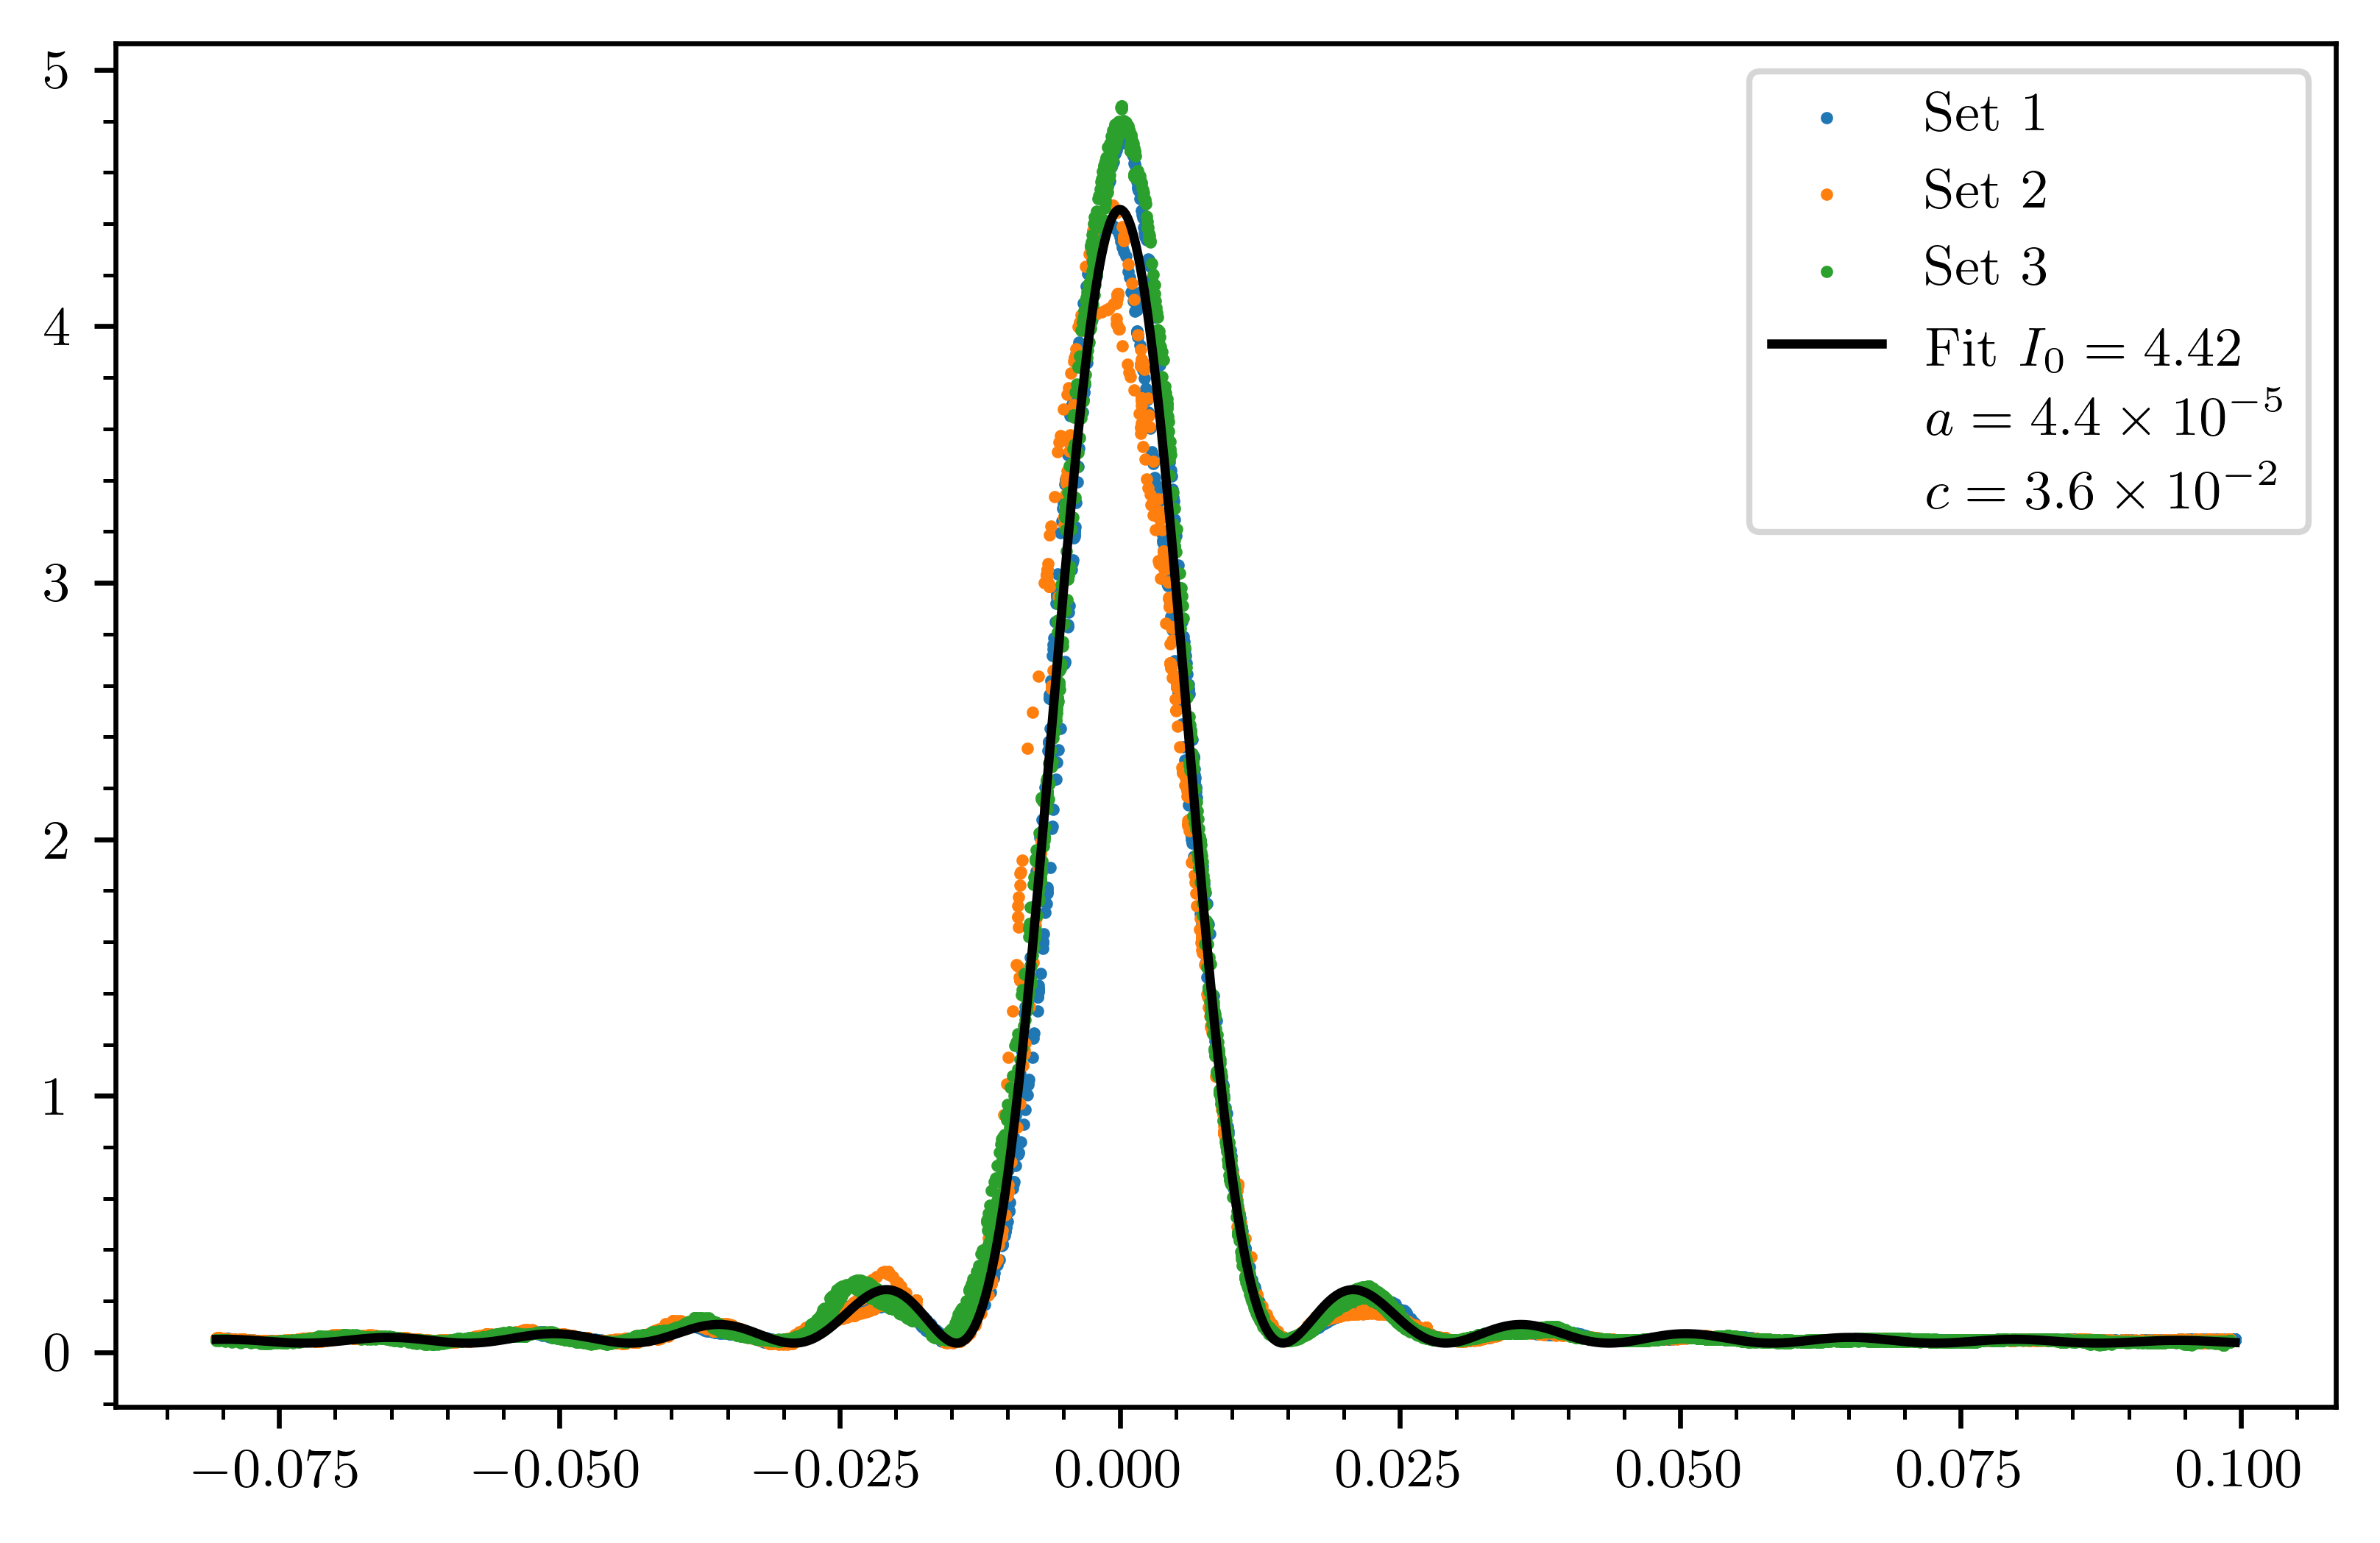
\includegraphics{fit_0.04.png}
    \caption{Intensità luminosa $I_{0}$ in funzione della posizione $y$ del sensore (in metri) per la fenditura a $\qty{0.04}{\mm}$. In figura è riportato il fit fatto utilizzando l'\autoref{eq:fit}. I valori dei parametri ottenuti sono $I_{0} = \num{4.42+-0.4}$, $a = \qty{4.4+-0.5e-5}{\mm}$ e $c = \num{3.60+-0.01}$. }
    \label{fig:fit 0.04}
\end{figure}

I valori di $a$ ottenuti dal grafico e dal fit risultano compatibili con il valore teorico.

Nel grafico seguente si confrontano i set ottenuti con le diverse aperture del sensore:

\begin{figure}[ht!]
    \centering
    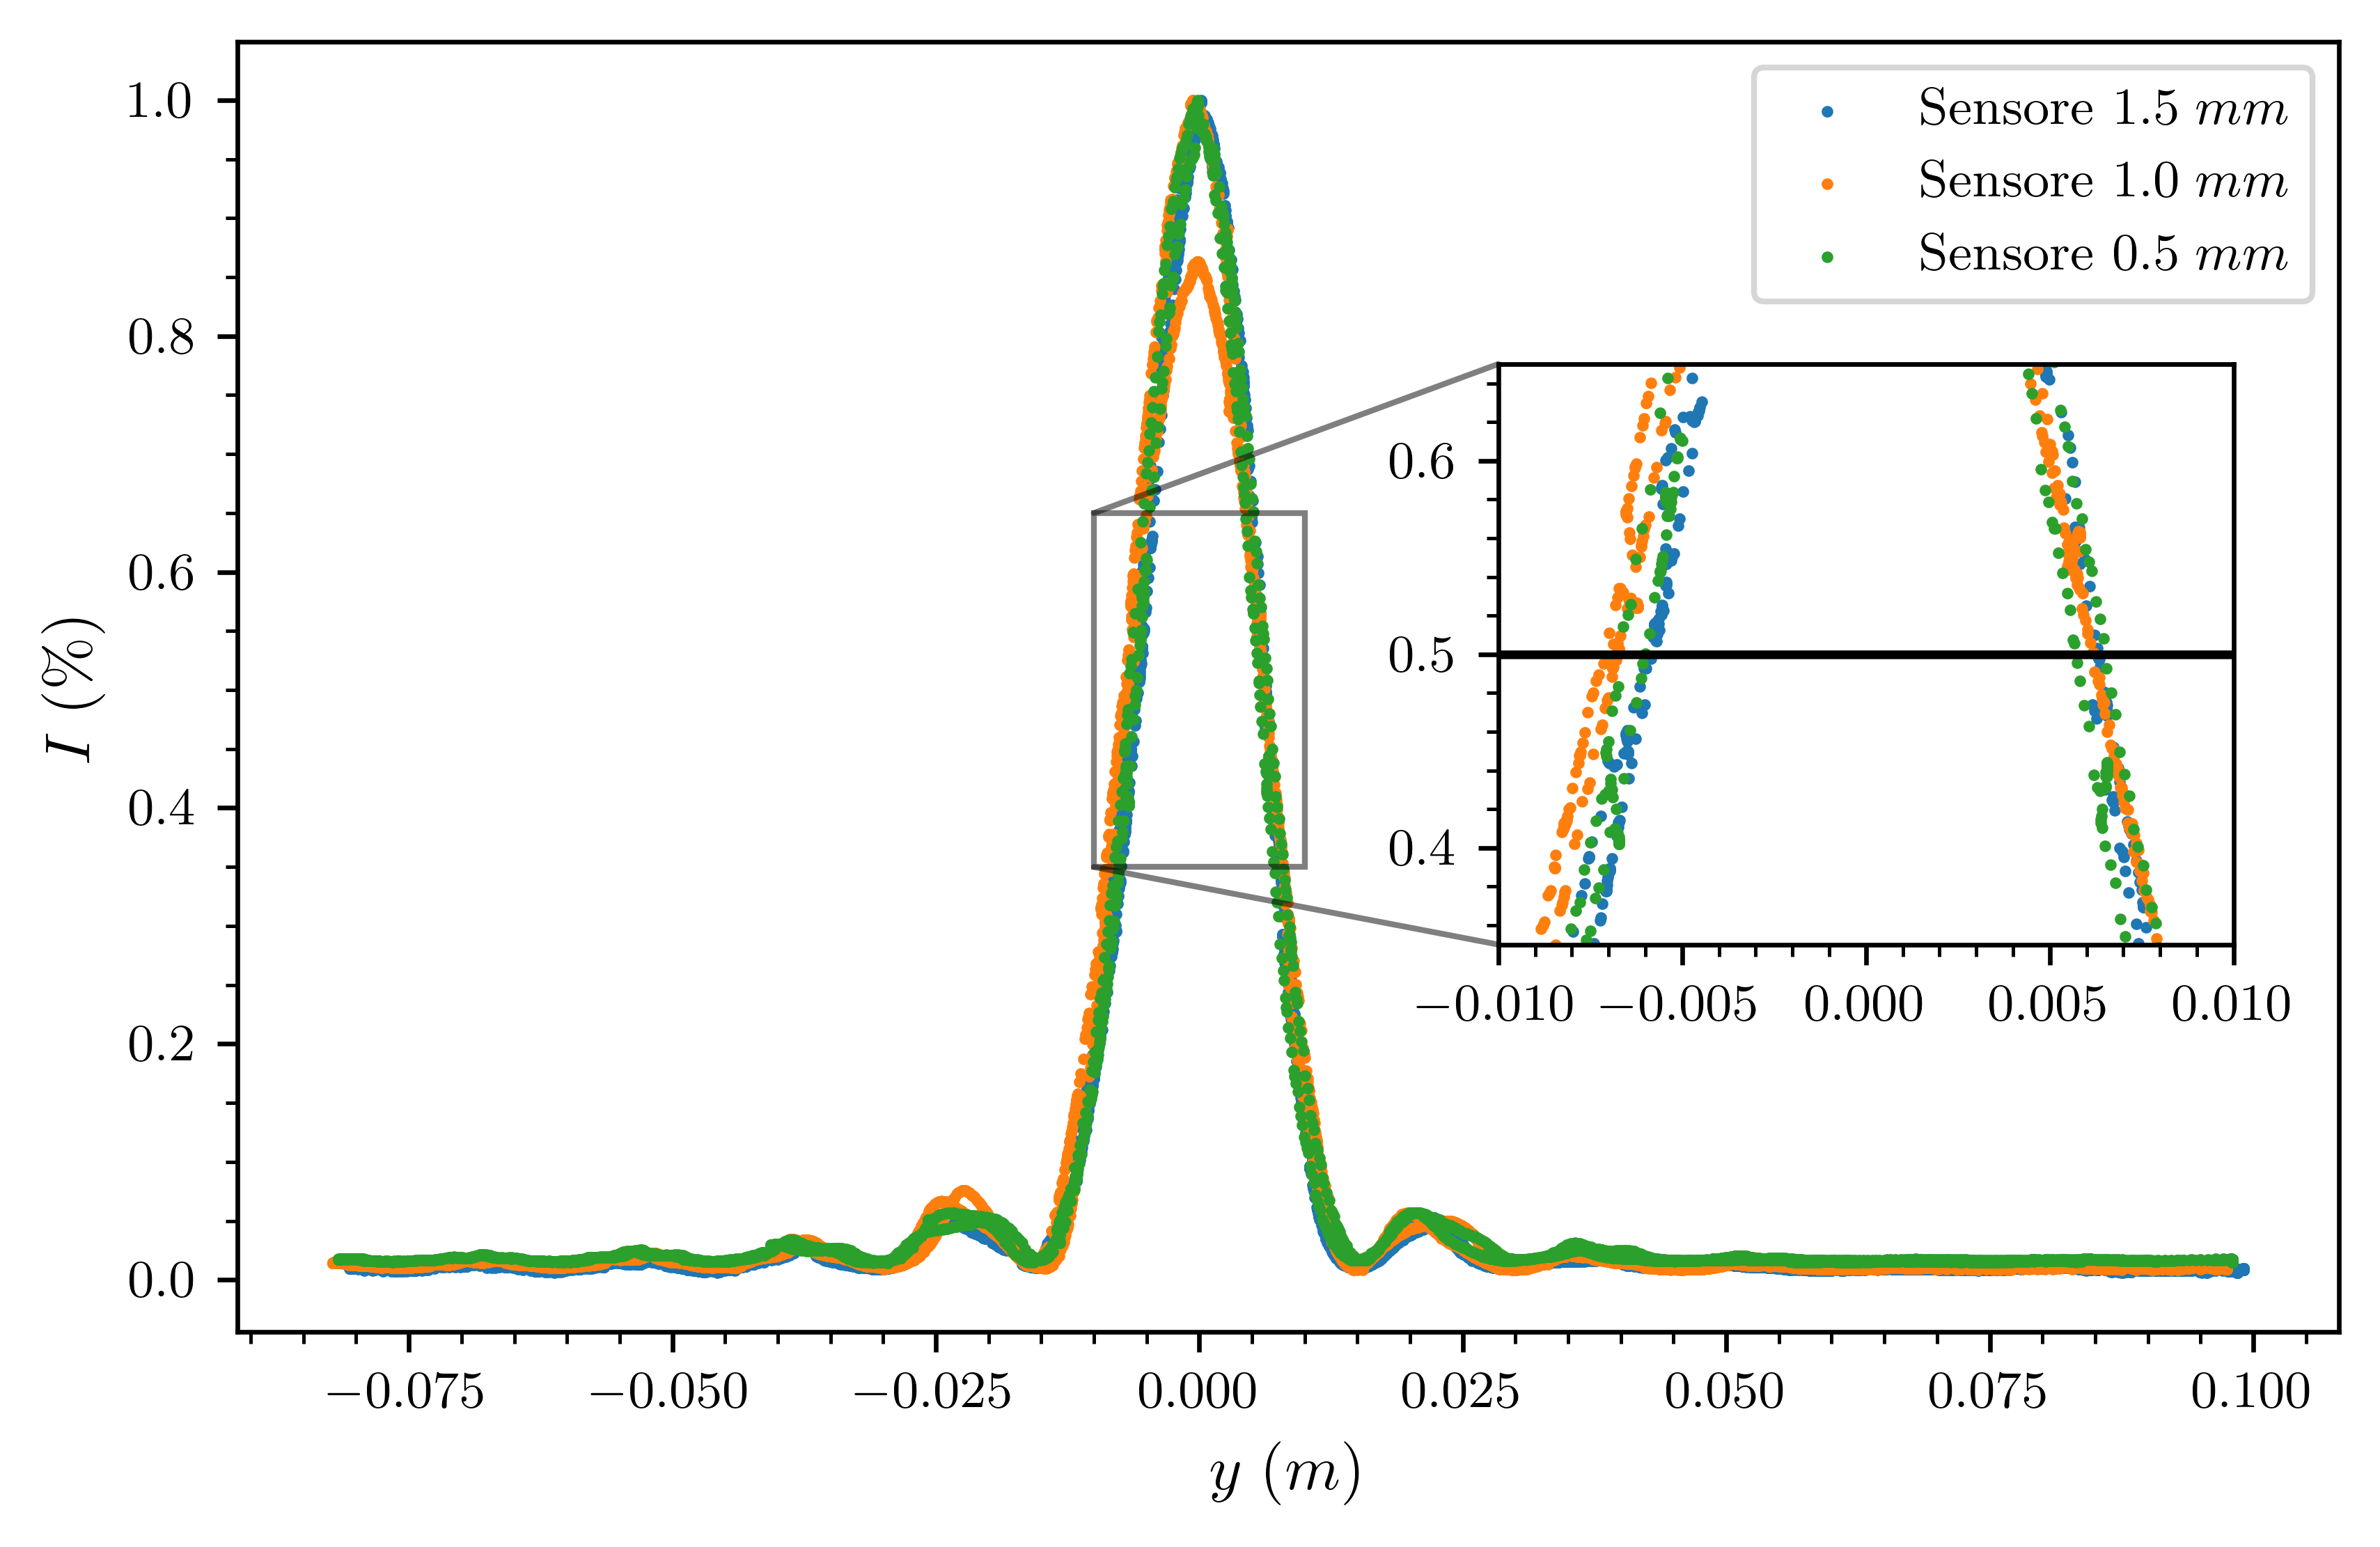
\includegraphics{sensor_0.04.png}
    \caption{Grafico dell'intensità luminosa relativa $I$ in funzione della posizione $y$ (in metri) per ciascuna delle tre aperture del sensore.} %! commento su rumore e confronto con il sensore 0.02
    \label{fig:sensore 0.04}
\end{figure}

\begin{figure}[ht!]
    \centering
    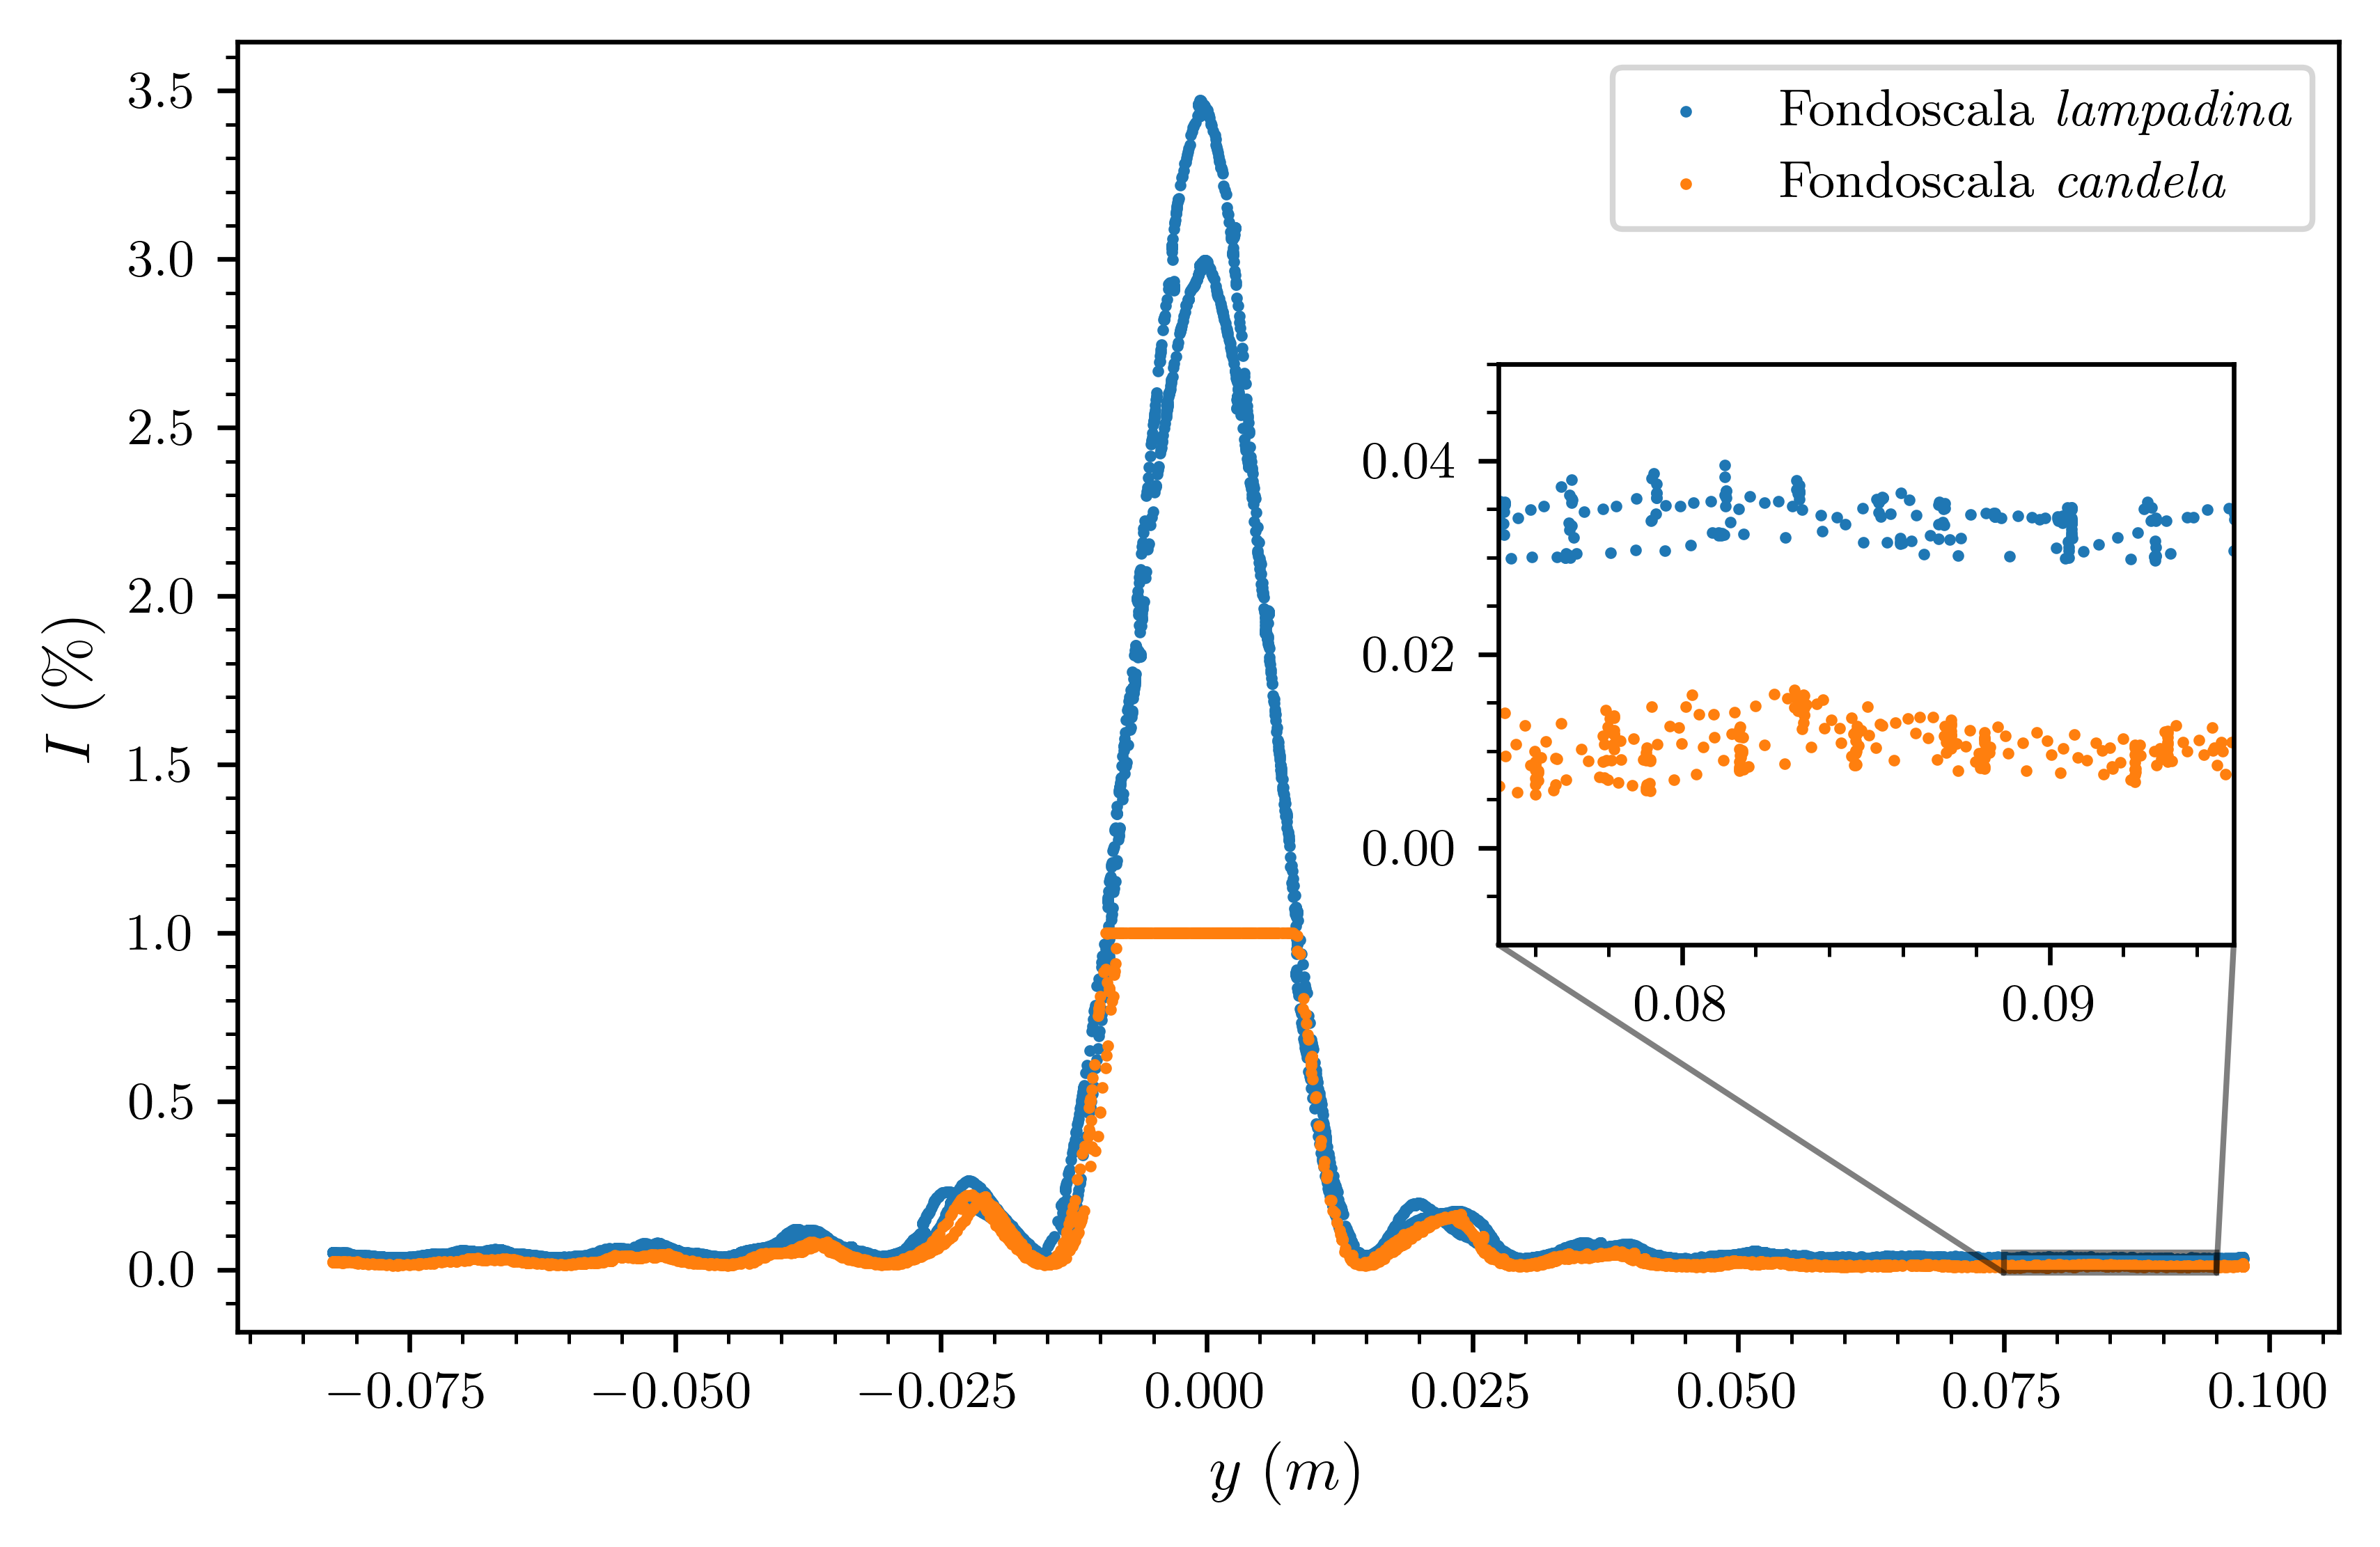
\includegraphics{scale_0.04.png}
    \caption{Grafico dell'intensità in funzione della posizione dove si confrontano i due fondoscala, con uno zoom sulla coda del grafico per evidenziare la diminuzione di rumore data dal fondoscala più piccolo.}
\end{figure}
\newpage

\subsection{Fenditura $a = \qty{0.08}{\milli\metre}$}

\begin{figure}[ht!]
    \centering
    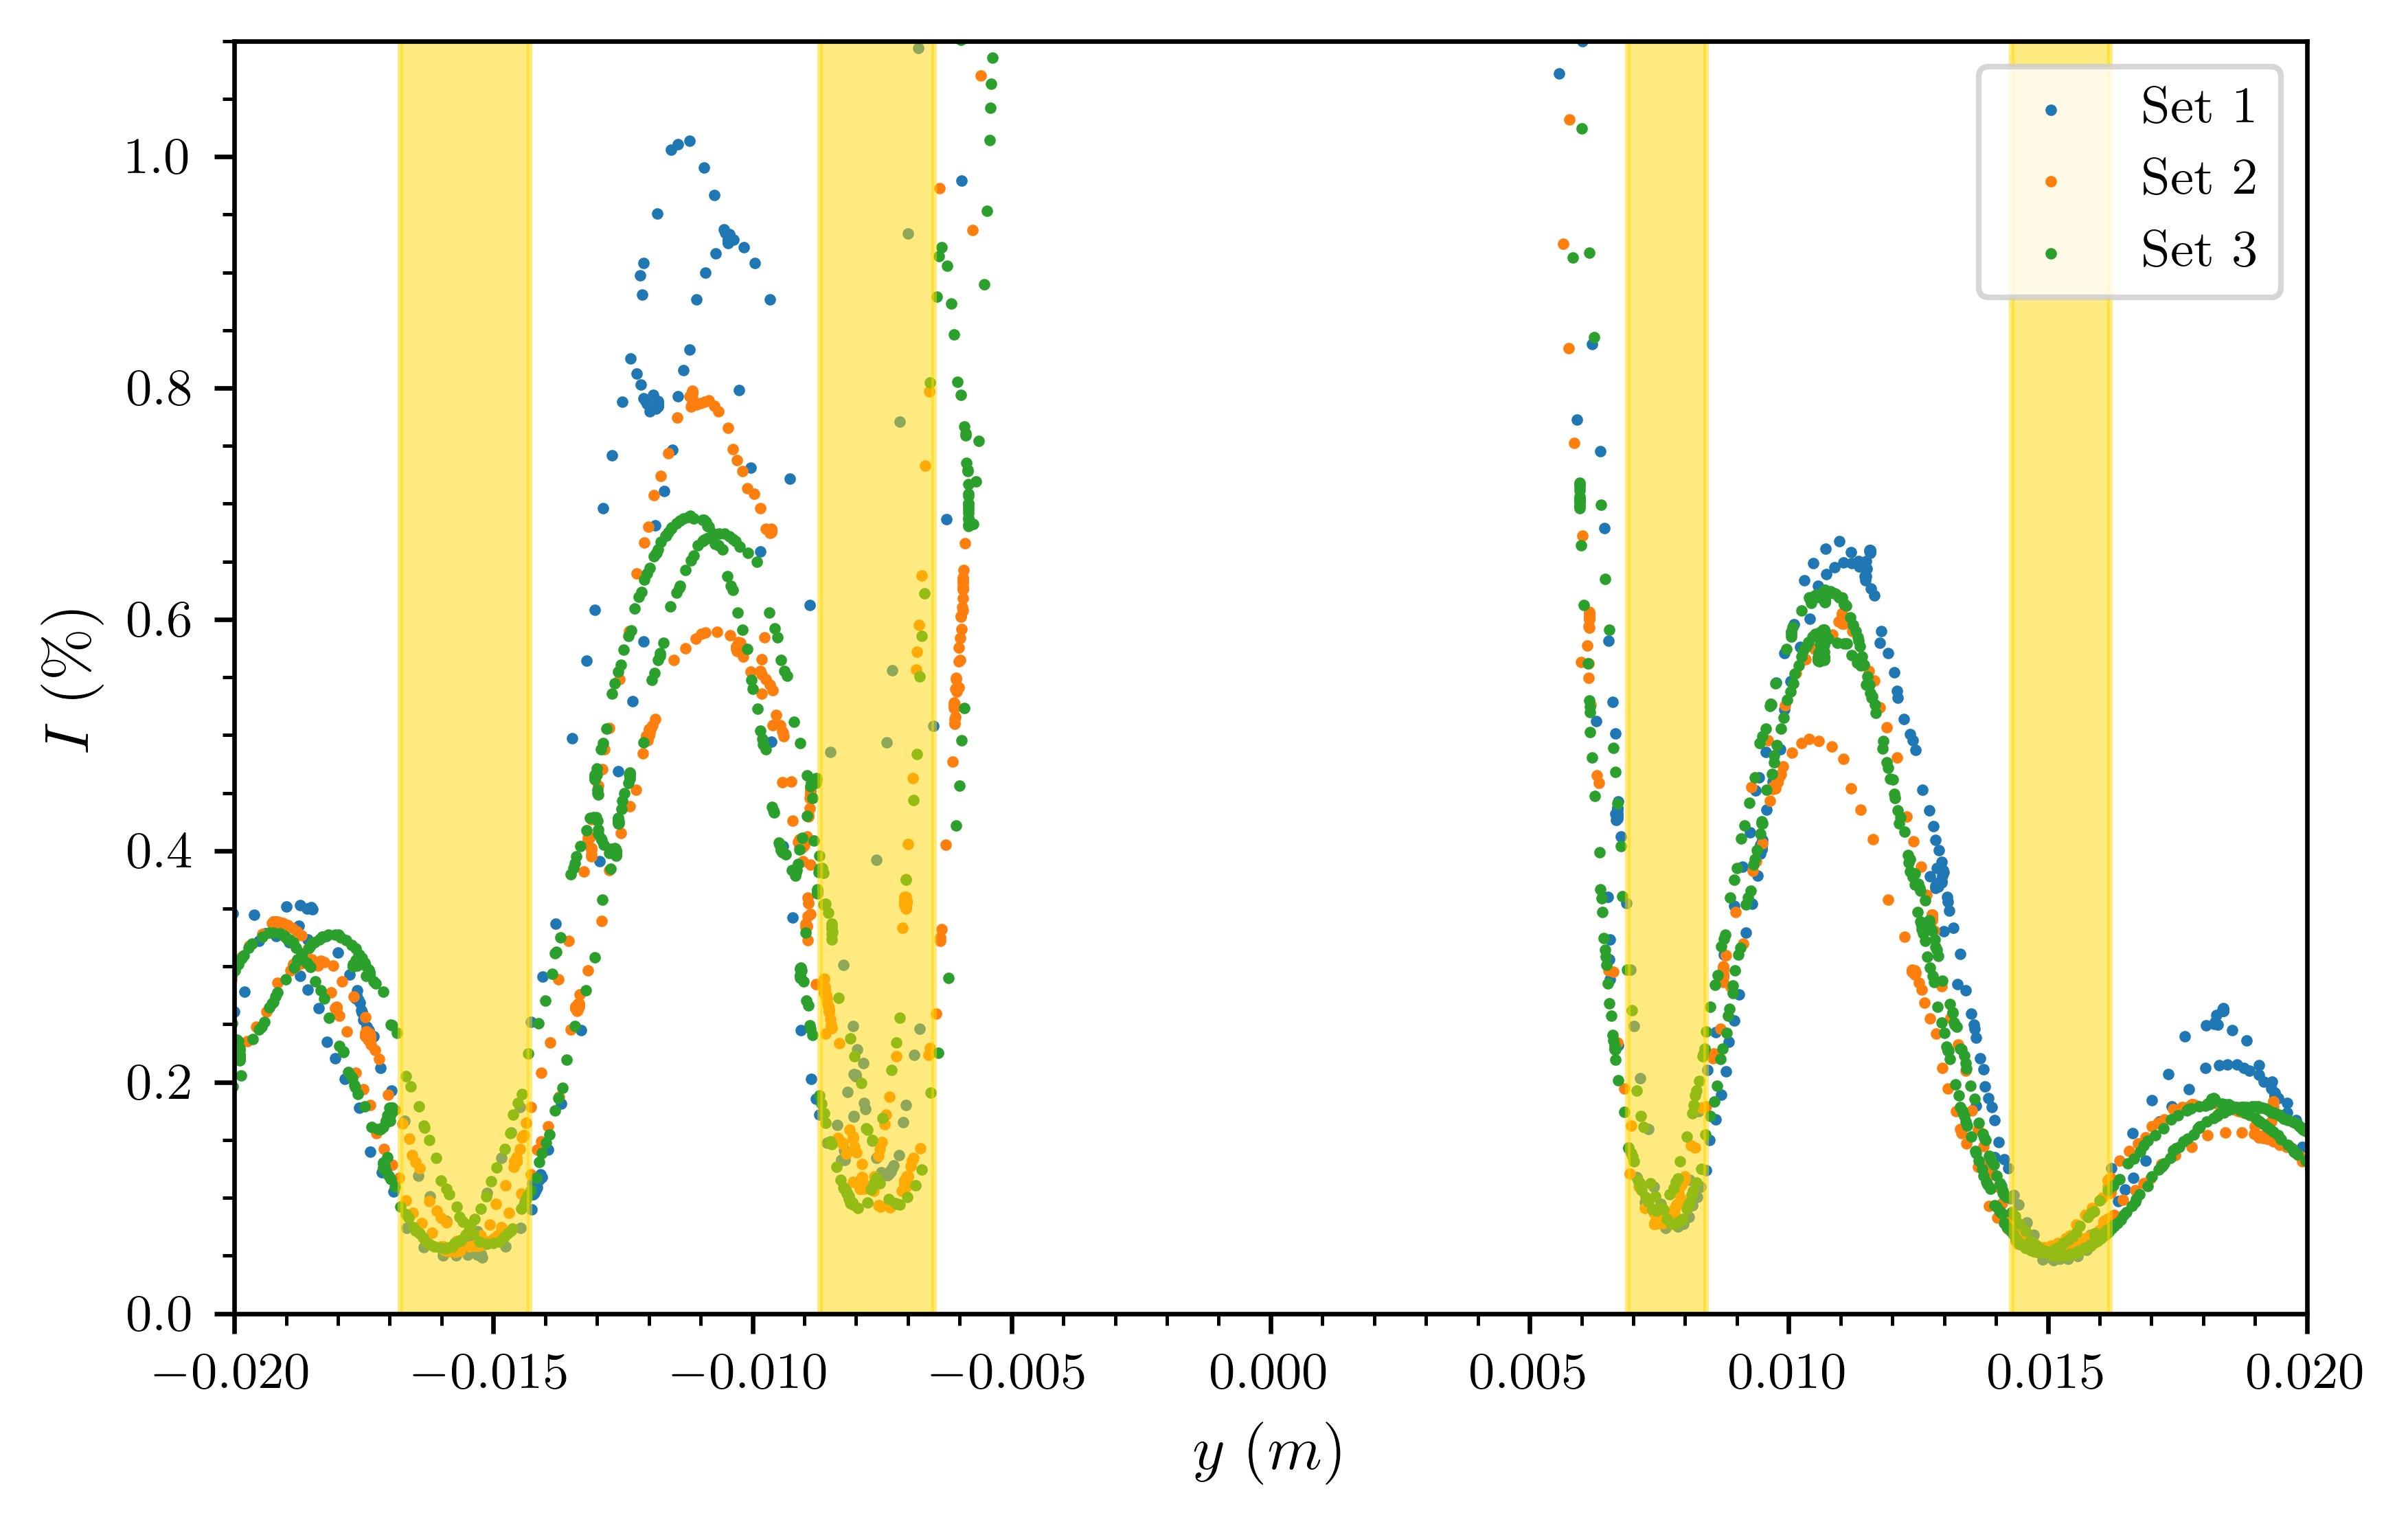
\includegraphics{min_0.08.png}
    \caption{Intensità luminosa $I$ in funzione della posizione $y$ del sensore (in metri) per la fenditura a $\qty{0.08}{\mm}$. I dati sono notevolmente asimmetrici, eccetto il set 3. In figura sono segnati i minimi ricavati graficamente con i relativi errori. Qui si considera un errore di posizione di $\qty{0.25}{\mm}$. %todo: aggiungere qualcosa in più alla descrizione + commentare simmetria (o assenza) dei set
    \label{fig:minimi 0.08}
\end{figure}

\begin{table}[ht!]
    \centering
    \caption{}
    \begin{tabular}{r|cc|c}
        \toprule
        $m$  & $y \; (\si{\metre})$ & $\frac{\lambda L}{a} \; (\si{\metre})$ & $a \; (\si{\mm})$ \\
        \midrule
        $-2$ & $0.0156 \pm 0.0013$ & $0.0078 \pm 0.0006$ & \num{0.082+-0.007} \\
        $-1$ & $0.0076 \pm 0.0011$ & $0.0076 \pm 0.0011$ & \num{0.084+-0.012} \\
        $1$  & $0.0077 \pm 0.0008$ & $0.0077 \pm 0.0008$ & \num{0.084+-0.008} \\
        $2$  & $0.0153 \pm 0.0010$ & $0.0076 \pm 0.0005$ & \num{0.084+-0.005} \\
        \bottomrule
    \end{tabular}
    \label{tab:minimi 0.08}
\end{table}

Intersecando i valori, si ottiene $a = 0.084 \pm 0.005$.

\begin{figure}[ht!]
    \centering
    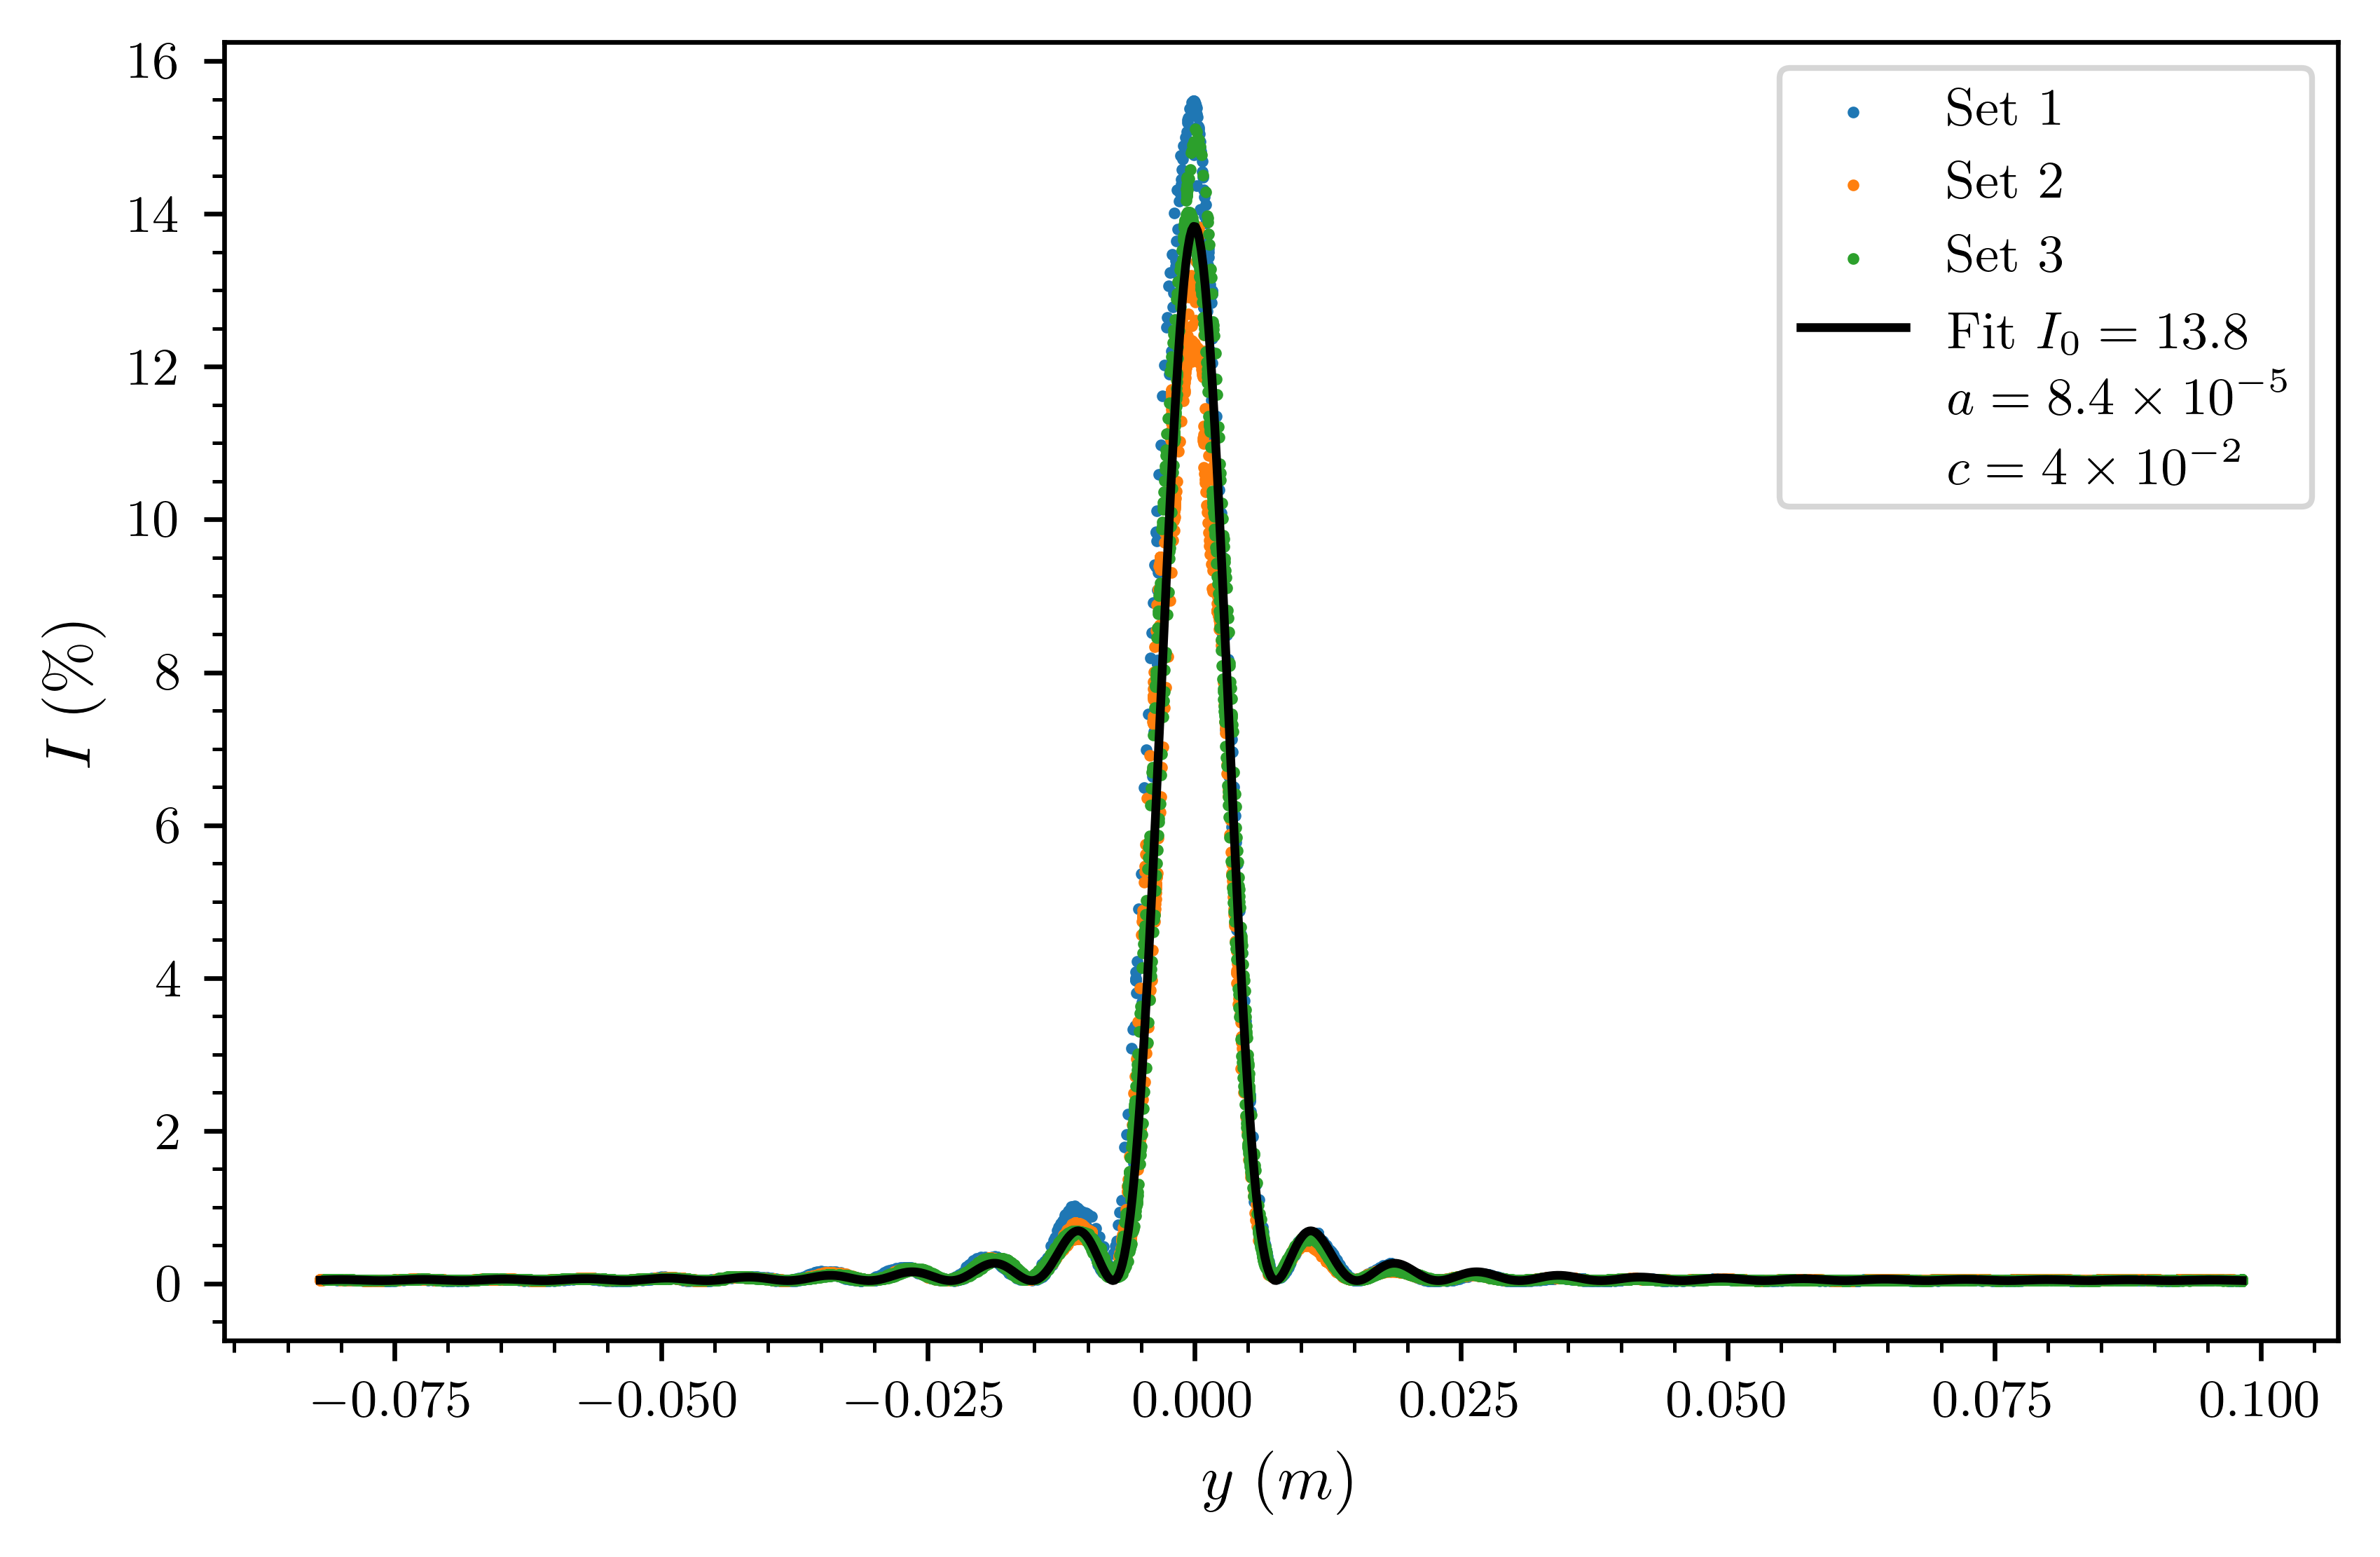
\includegraphics{fit_0.08.png}
    \caption{Intensità luminosa $I_{0}$ in funzione della posizione $y$ del sensore (in metri) per la fenditura a $\qty{0.08}{\mm}$. In figura è riportato il fit fatto utilizzando l'\autoref{eq:fit}. I valori dei parametri ottenuti sono $I_{0} = \num{13.8+-1.6}$, $a = \qty{8.4+-0.4e-5}{\mm}$ e $c = \num{4+-1.2e-2}$. }
    \label{fig:fit 0.08}
\end{figure}

I valori di $a$ ottenuti dal grafico e dal fit risultano compatibili con il valore teorico.

Anche qui si confrontano i dati ottenuti con ciascuna delle due aperture:

% \begin{figure}[ht!]
%     \centering
%     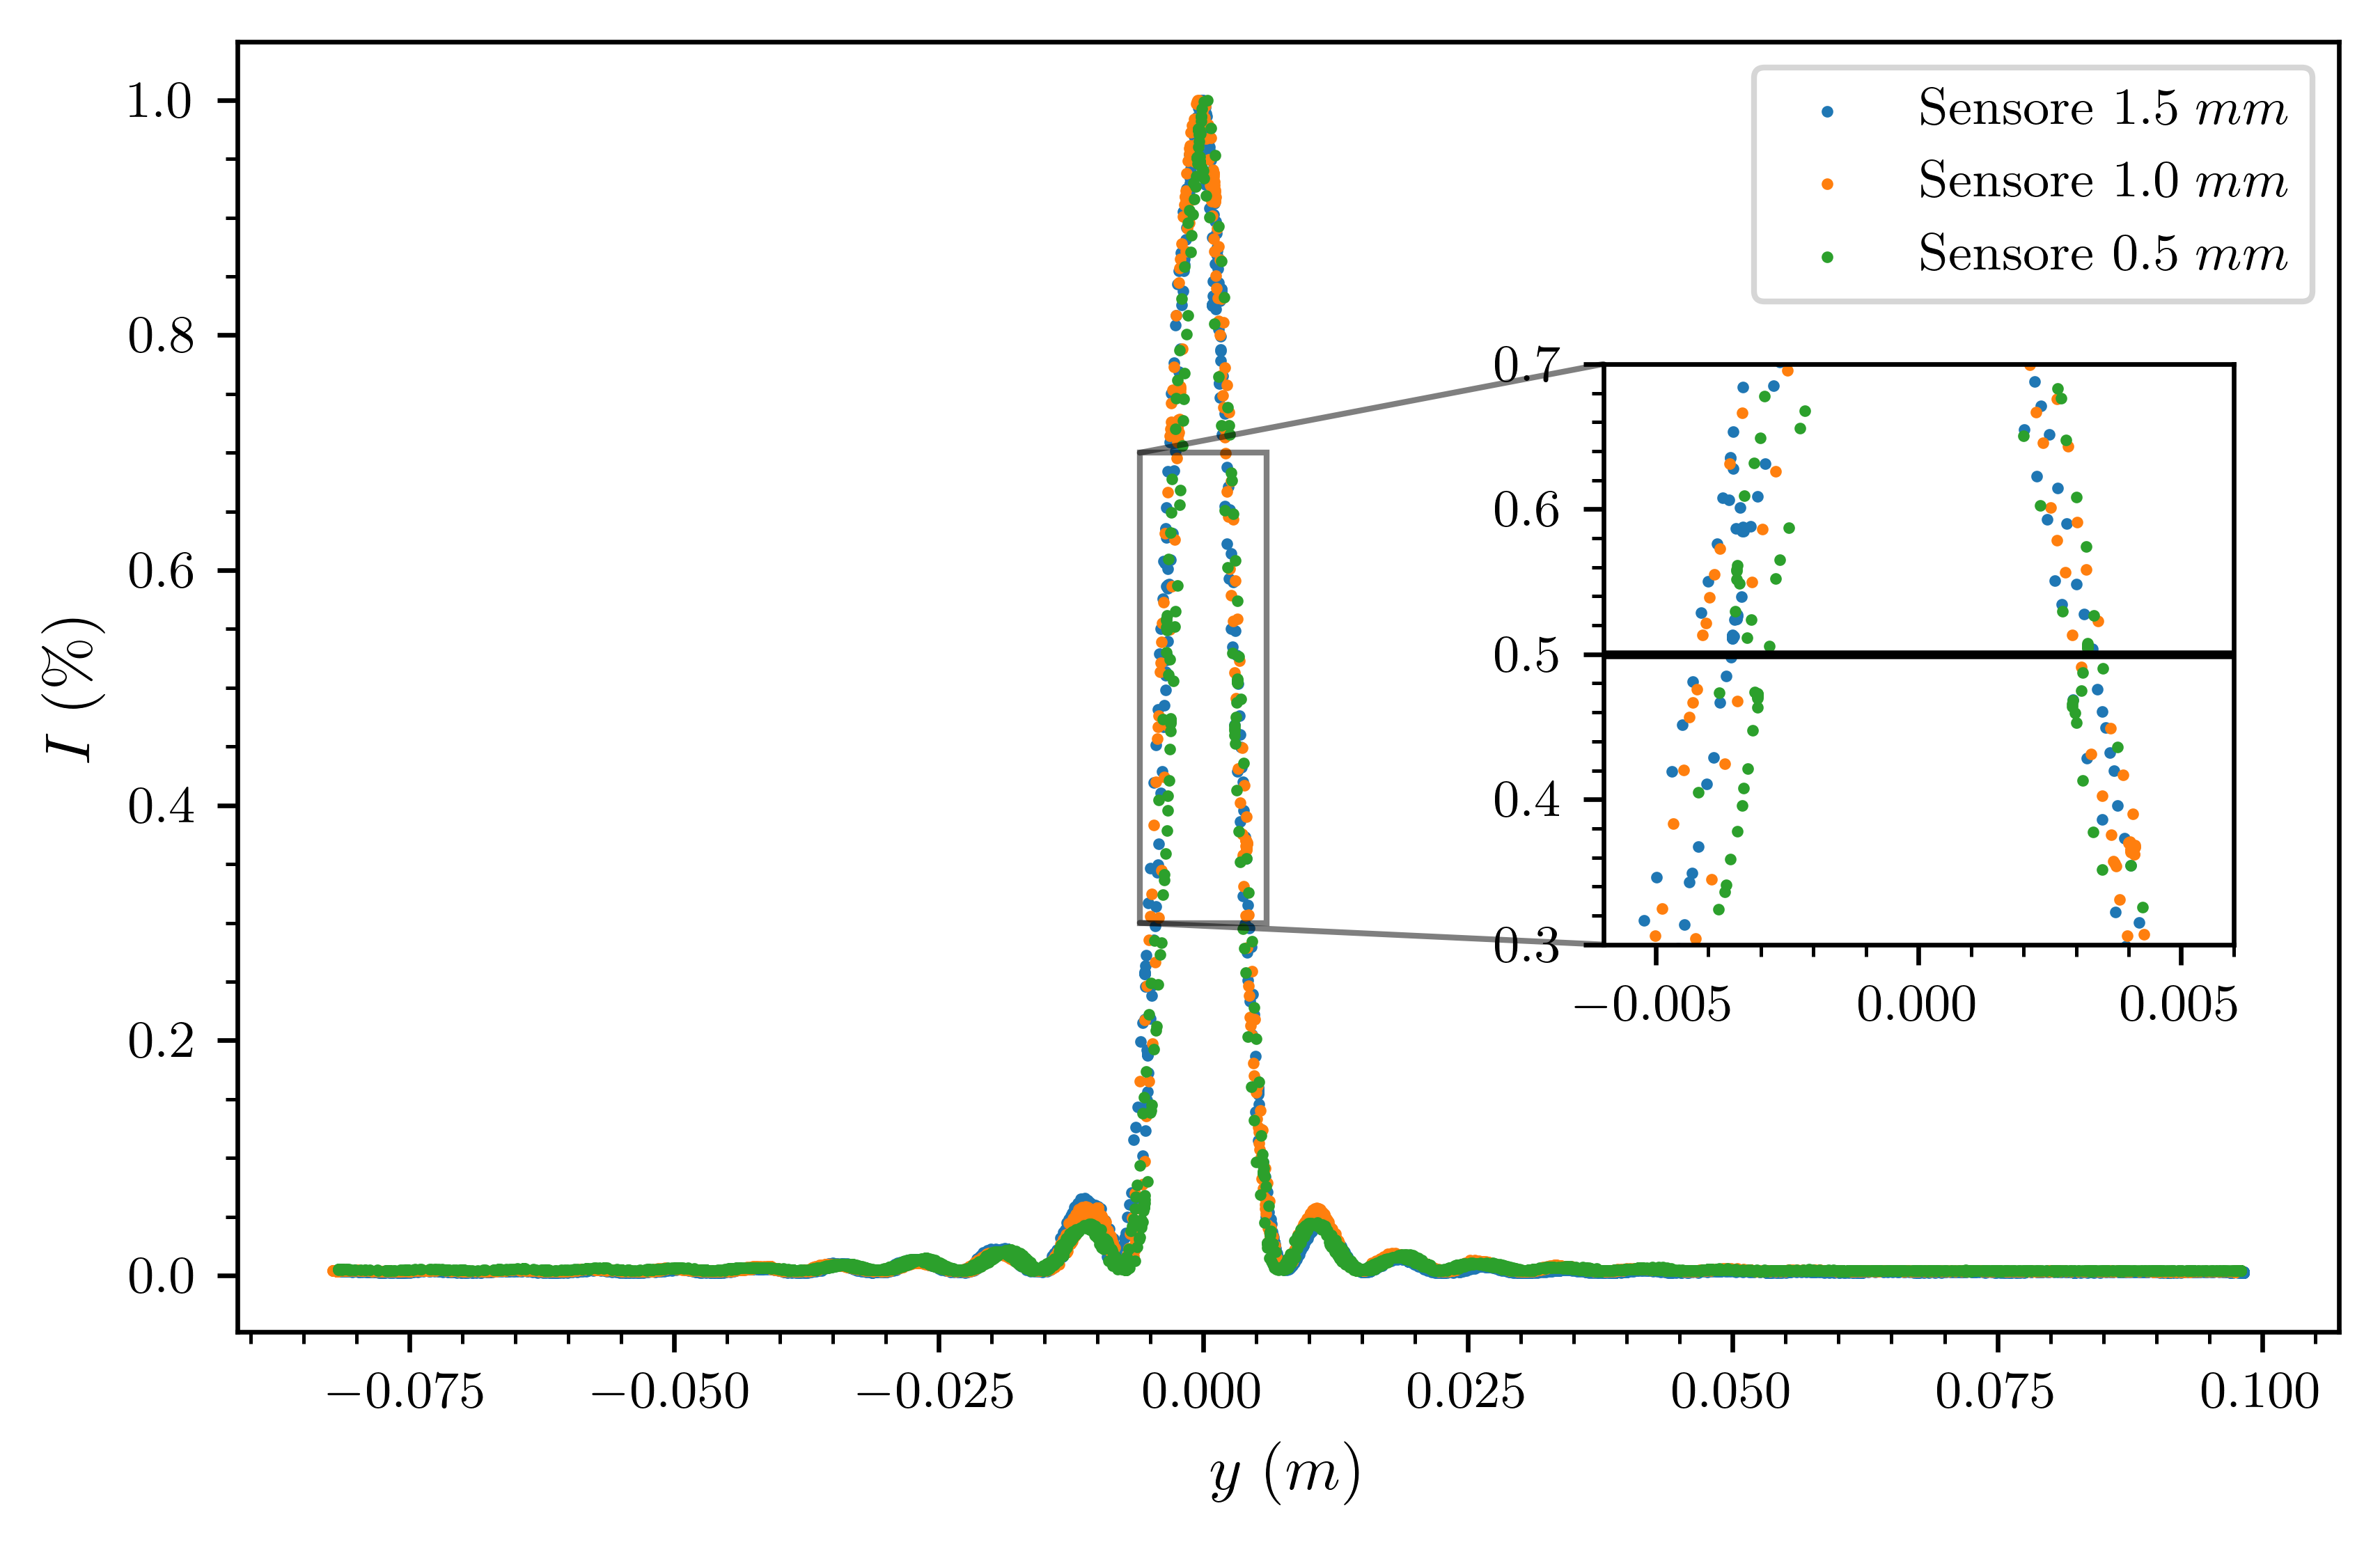
\includegraphics{sensor_0.08.png}
%     \caption{Grafico dell'intensità luminosa relativa $I$ in funzione della posizione $y$ (in metri) per ciascuna delle due aperture del sensore.} %! commento su rumore e confronto con il sensore 0.02
%     \label{fig:sensore 0.08}
% \end{figure}

\end{document}